% *******************************************************************
% STOP - Bitte zuerst lesen, bevor Sie weitermachen
%
% Einige Dinge müssen Sie an Ihre Bedürfnisse (und die Vorgaben Ihres
% Betreuers anpassen).
%
% 1. Sprache
% Das Template unterstützt Deutsch und Englisch, Standard ist Deutsch.
% Wenn Sie Englisch verwenden wollen, ändern Sie bitte direkt am Anfang
% dieser Datei den Eintrag
%    \newcommand{\hsmasprache}{de}
% auf
%    \newcommand{\hsmasprache}{en}
%
% 2. Zitierstil
% Abhängig von dem gewünschten Zitierstil passen Sie bitte in
% preambel.tex die Einstellungen bei \usepackage[backend=biber...
% an. Wie ist dort genau erklärt.
% Achtung: Wenn Sie als Zitierstil Fußnoten wählen bzw. generell
% -------  mit Fußnoten arbeiten, dann beachten Sie bitte, dass
%          Fußnoten in Bildunterschriften und Tabellenüberschriften
%          nicht funktionieren.
%          Siehe hierzu https://texfaq.org/FAQ-ftncapt
%          und https://texfaq.org/FAQ-footintab
%          Sinnvollerweise verzichten Sie auf Fußnoten an diesen
%          Stellen und fügen Quellen einfach per \parancite ein.
%
% 3. Doppelseitiger oder einseitiger Druck
% Das Template ist für doppelseitigen Druck eingestellt. Wollen Sie
% einseitig drucken, müssen Sie in preambel.tex die Einstellungen
% für \documentclass ändern. Und zwar von twoside=on auf twoside=off.
%
% 4. Abkürzungen auf richtige Breite einstellen und sortieren
% In der Datei kapitel/abkuerzungen.tex müssen Sie die _längste_
% Abkürzung in die eckigen Klammern von \begin{acronym} schreiben,
% sonst werden die Abkürzungen nicht richtig ausgerichtet.
% Also z.B. \begin{acronym}[DSGVO].
% Außerdem müssen Sie die Abkürzungen selbst (manuell) sortieren,
% da dies nicht automatisch passiert. Am einfachsten verwenden Sie
% hierzu die Sortierfunktion Ihres Texteditors.
%
% 5. Unnötige Teile entfernen
% Entfernen Sie die Teile, die Sie nicht brauchen, z.B. Anhänge,
% Quelltextverzeichnis etc. Siehe unten
%
% 6. Silbentrennung
% LaTeX führt eine automatische Silbentrennung durch. Allerdings
% werden Wörter, die bereits einen Bindestrich enthalten nicht
% getrennt, z.B. Datenschutz-Grundverordnung. Wenn Sie Ihren Text auf
% Deutsch schreiben, können Sie dann alternativ "= für den Bindestrich
% im Wort verwenden, z.B. Datenschutz"=Grundverordnung, damit LaTeX
% weiterhin richtig trennt.
% Ist die Silbentrennung aus einem anderen Grund nicht erfolgt, sodass
% das Wort über den rechten Rand hinaussteht oder wenn Sie eine weitere
% Trennstelle wollen, können Sie LaTeX helfen, indem Sie weitere
% Trennstellen angeben. Dies geschieht durch "- als Zeichen, z.B.
% Staats"-vertrag.
%
% 7. Nummerierung der Fußnoten
% LaTeX beginnt die Nummerierung der Fußnoten in jedem Kapitel wieder
% bei 1. Manche Dozenten wollen aber eine durchlaufende Nummerierung
% über die gesamte Arbeit. In diesem Fall gehen Sie in die preambel.tex
% und kommentieren den Befehl \counterwithout{footnote}{chapter} ein.
% *******************************************************************

% Sprache für das Dokument festlegen
\newcommand{\hsmasprache}{de} % de oder en für Deutsch oder Englisch

% Preambel mit Einstellungen importieren
% Dokumententyp und benutzte Pakete
\documentclass[open=right,  % Kapitel darf nur auf rechten Seite beginnen
  paper=a4,               % DIN-A4-Papier
  fontsize=12pt,          % Schriftgöße
  headings=small,         % Kleine Überschriften
  headsepline=true,       % Trennlinie am Kopf der Seite
  footsepline=false,      % Keine Trennlinie am Fuß der Seite
  bibliography=totoc,     % Literaturverzeichnis in das Inhaltsverzeichnis aufnehmen
  twoside=on,             % Doppelseitiger Druck - auf off stellen für einseitig
  DIV=7,                  % Verhältnis der Ränder zum bedruckten Bereich
  chapterprefix=true,     % Kapitel x vor dem Kapitelnamen
  cleardoublepage=plain]{scrbook}

% Pakete einbinden, die benötigt werden
\usepackage{ifthen}               % Logische Bedingungen mit ifthenelse
\usepackage{scrlayer-scrpage}
\usepackage[utf8]{inputenc}       % Dateien in UTF-8 benutzen
\usepackage[T1]{fontenc}          % Zeichenkodierung
\usepackage{graphicx}             % Bilder einbinden
\usepackage{enumitem}             % Eigene Listen definieren können

% Setzen von Optionen abhängig von der gewählten Sprache. Die Sprache wird
% in thesis.tex gesetzt.
\ifthenelse{\equal{\hsmasprache}{de}}%
{%
  \usepackage[main=ngerman, english]{babel}  % Deutsche Sprachunterstützung
  \usepackage[autostyle=true,german=quotes]{csquotes} % Deutsche Anführungszeichen
  \usepackage[pagebackref=false,german]{hyperref} % Hyperlinks
  \newcommand{\hsmasortlocale}{de_DE} % Sortierung der Literatur
}%
{%
  \usepackage[main=english, ngerman]{babel} % Englische Sprachunterstützung
  \usepackage[autostyle=true,english=american]{csquotes} % Englische Anführungszeichen
  \usepackage[pagebackref=false,english]{hyperref}  % Hyperlinks
  \newcommand{\hsmasortlocale}{en_US} % Sortierung der Literatur
}%

\usepackage{xcolor}               % Unterstützung für Farben
\usepackage{amsmath}              % Mathematische Formeln
\usepackage{amsfonts}             % Mathematische Zeichensätze
\usepackage{amssymb}              % Mathematische Symbole
\usepackage{float}                % Fließende Objekte (Tabellen, Grafiken etc.)
\usepackage{booktabs}             % Korrekter Tabellensatz
\usepackage[printonlyused]{acronym}  % Abkürzungsverzeichnis [nur verwendete Abkürzungen]
\usepackage{makeidx}              % Sachregister
\usepackage{listings}             % Quelltexte
\usepackage{listingsutf8}         % Quelltexte in UTF8
\usepackage[hang,font={sf,footnotesize},labelfont={footnotesize,bf}]{caption} % Beschriftungen
\usepackage[scaled]{helvet}       % Schrift Helvetia laden
\usepackage[absolute]{textpos}    % Absolute Textpositionen (für Deckblatt)
\usepackage{calc}                 % Berechnung von Positionen
\usepackage{blindtext}            % Blindtexte
\usepackage[bottom=40mm,left=35mm,right=35mm,top=30mm]{geometry} % Ränder ändern
\usepackage{setspace}             % Abstände korrigieren
\usepackage{scrhack}              % tocbasic Warnung entfernen
\usepackage[all]{hypcap}          % Korrekte Verlinkung von Floats
\usepackage{tabularx}             % Spezielle Tabellen
\usepackage[backend=biber,
  isbn=false,                     % ISBN nicht anzeigen, gleiches geht mit nahezu allen anderen Feldern
  sortlocale=\hsmasortlocale,     % Sortierung der Einträge für Deutsch
  %      de_DE: für Deutsch
  %      en_US: für Englisch
  autocite=inline,                % regelt Aussehen für \autocite
  %      inline: Zitat in Klammern (\parancite)
  %      footnote: Zitat in Fußnoten (\footcite)
  %      plain: Zitat direkt ohne Klammern (\cite)
  style=ieee,               % Legt den Stil für die Zitate fest
  %      ieee: Zitate als Zahlen [1]
  %      alphabetic: Zitate als Kürzel und Jahr [Ein05]
  %      authoryear: Zitate Author und Jahr [Einstein (1905)]
  hyperref=true,                  % Hyperlinks für Zitate
  firstinits=false                % Vornamen abkürzen (Maier, M. anstatt Maier, Markus)?
  %      true: abkürzen
  %      false: nicht abkürzen
]{biblatex}                       % Literaturverwaltung mit BibLaTeX
\usepackage{rotating}             % Seiten drehen
\usepackage{harveyballs}          % Harveyballs
\usepackage{chngcntr}             % Counter (Zähler) ändern können - für Fußnotennummern

% Einstellungen zu den Fußnoten
\renewcommand{\footnotesize}{\fontsize{9}{10}\selectfont} % Größe der Fußnoten
\setlength{\footnotesep}{8pt} % Abstand zwischen den Fußnoten

% Kommentieren Sie diese Zeile ein, wenn Sie eine "durchlaufende" Nummerierung bei den
% Fußnoten wünschen, d.h. wenn die Fußnoten nicht bei jedem Kapitel wieder bei 1
% beginnen sollen.
%\counterwithout{footnote}{chapter}

\setlength{\bibitemsep}{1em}      % Abstand zwischen den Literaturangaben
\setlength{\bibhang}{2em}         % Einzug nach jeweils erster Zeile

% Trennung von URLs im Literaturverzeichnis (große Werte [> 10000] verhindern die Trennung)
\defcounter{biburlnumpenalty}{10} % Strafe für Trennung in URL nach Zahl
\defcounter{biburlucpenalty}{500} % Strafe für Trennung in URL nach Großbuchstaben
\defcounter{biburllcpenalty}{500} % Strafe für Trennung in URL nach Kleinbuchstaben

% Farben definieren
\definecolor{linkblue}{RGB}{0, 0, 100}
\definecolor{linkblack}{RGB}{0, 0, 0}
\definecolor{comment}{RGB}{63, 127, 95}
\definecolor{darkgreen}{RGB}{14, 144, 102}
\definecolor{darkblue}{RGB}{0,0,168}
\definecolor{darkred}{RGB}{128,0,0}
\definecolor{javadoccomment}{RGB}{0,0,240}

% Einstellungen für das Hyperlink-Paket
\hypersetup{
  colorlinks=true,      % Farbige links verwenden
  %    allcolors=linkblue,
  linktoc=all,          % Links im Inhaltsverzeichnis
  linkcolor=linkblack,  % Querverweise
  citecolor=linkblack,  % Literaturangaben
  filecolor=linkblack,  % Dateilinks
  urlcolor=linkblack    % URLs
}

\definecolor{codegreen}{rgb}{0,0.6,0}
\definecolor{codegray}{rgb}{0.5,0.5,0.5}
\definecolor{codepurple}{rgb}{0.58,0,0.82}
\definecolor{backcolour}{rgb}{0.95,0.95,0.92}

\lstdefinestyle{mystyle}{
  backgroundcolor=\color{backcolour},
  commentstyle=\color{codegreen},
  keywordstyle=\color{magenta},
  numberstyle=\tiny\color{codegray},
  stringstyle=\color{codepurple},
  basicstyle=\ttfamily\footnotesize,
  breakatwhitespace=false,
  breaklines=true,
  captionpos=b,
  keepspaces=true,
  numbers=left,
  numbersep=5pt,
  showspaces=false,
  showstringspaces=false,
  showtabs=false,
  tabsize=2
}
\lstset{style=mystyle}

% % Einstellungen für Quelltexte
% \lstset{
% xleftmargin=0.2cm,
% basicstyle=\footnotesize\ttfamily,
% keywordstyle=\color{darkgreen},
% identifierstyle=\color{darkblue},
% commentstyle=\color{comment},
% stringstyle=\color{darkred},
% tabsize=2,
% lineskip={2pt},
% columns=flexible,
% inputencoding=utf8,
% captionpos=b,
% breakautoindent=true,
% breakindent=2em,
% breaklines=true,
% prebreak=,
% postbreak=,
% numbers=none,
% numberstyle=\tiny,
% showspaces=false,      % Keine Leerzeichensymbole
% showtabs=false,        % Keine Tabsymbole
% showstringspaces=false,% Leerzeichen in Strings
% morecomment=[s][\color{javadoccomment}]{/**}{*/},
% literate={Ö}{{\"O}}1 {Ä}{{\"A}}1 {Ü}{{\"U}}1 {ß}{{\ss}}2 {ü}{{\"u}}1 {ä}{{\"a}}1 {ö}{{\"o}}1
% }

\urlstyle{same}

% Einstellungen für Überschriften
\renewcommand*{\chapterformat}{%
  \Large\chapapp~\thechapter   % Große Schrift
  \vspace{0.3cm}               % Abstand zum Titel des Kapitels
}

% Abstände für die Überschriften setzen
\renewcommand{\chapterheadstartvskip}{\vspace*{2.6cm}}
\renewcommand{\chapterheadendvskip}{\vspace*{1.5cm}}

% Vertikale Abstände für die Überschriften etwas verkleinern
\RedeclareSectionCommand[
  beforeskip=-1.8\baselineskip,
  afterskip=0.25\baselineskip]{section}

\RedeclareSectionCommand[
  beforeskip=-1.8\baselineskip,
  afterskip=0.15\baselineskip]{subsection}

\RedeclareSectionCommand[
  beforeskip=-1.8\baselineskip,
  afterskip=0.15\baselineskip]{subsubsection}

% In der Kopfzeile nur die kurze Kapitelbezeichnung (ohne Kapitel davor)
\renewcommand*\chaptermarkformat{\thechapter\autodot\enskip}
\automark[chapter]{chapter}

% Einstellungen für Schriftarten
\setkomafont{pagehead}{\normalfont\sffamily}
\setkomafont{pagenumber}{\normalfont\sffamily}
\setkomafont{paragraph}{\sffamily\bfseries\small}
\setkomafont{subsubsection}{\sffamily\itshape\bfseries\small}
\addtokomafont{footnote}{\footnotesize}
\setkomafont{chapter}{\LARGE\selectfont\bfseries}

% Wichtige Abstände
\setlength{\parskip}{0.2cm}  % 2mm Abstand zwischen zwei Absätzen
\setlength{\parindent}{0mm}  % Absätze nicht einziehen
\clubpenalty = 10000         % Keine "Schusterjungen"
\widowpenalty = 10000        % Keine "Hurenkinder"
\displaywidowpenalty = 10000 % Keine "Hurenkinder"
% Siehe: https://de.wikipedia.org/wiki/Hurenkind_und_Schusterjunge

% Index erzeugen
\makeindex

% Einfacher Font-Wechsel über dieses Makro
\newcommand{\changefont}[3]{
  \fontfamily{#1} \fontseries{#2} \fontshape{#3} \selectfont}

% Eigenes Makro für Bilder. Das label (für \ref) ist dann einfach
% der Name der Bilddatei
\newcommand{\bild}[3]{
  \begin{figure}[ht]
    \centering
    \includegraphics[width=#2]{#1}
    \caption{#3}
    \label{#1}
  \end{figure}}

% Wo liegt Sourcecode?
\newcommand{\srcloc}{src/}

% Wo sind die Bilder?
\graphicspath{{bilder/}}

% Makros für typographisch korrekte Abkürzungen
\newcommand{\zb}[0]{z.\,B.}
\newcommand{\dahe}[0]{d.\,h.}
\newcommand{\ua}[0]{u.\,a.}

% Flags für Veröffentlichung und Sperrvermerk
\newboolean{hsmapublizieren}
\newboolean{hsmasperrvermerk}

% Tabellenzellen mit mehreren Zeilen
\newcolumntype{L}{>{\raggedright\arraybackslash}X}
\newcolumntype{b}{l}
\newcolumntype{s}{>{\hsize=.3\hsize}l}
\newcolumntype{F}{>{\hsize=\dimexpr2\hsize+2\tabcolsep+\arrayrulewidth\relax}X}

% Checklisten mit zwei Ebenen
\newlist{checklist}{itemize}{2}
\setlist[checklist]{label=$\square$}

% Dokumenteninfos importieren
% -------------------------------------------------------
% Daten für die Arbeit
% Wenn hier alles korrekt eingetragen wurde, wird das Titelblatt
% automatisch generiert. D.h. die Datei titelblatt.tex muss nicht mehr
% angepasst werden.

% Titel der Arbeit auf Deutsch
\newcommand{\hsmatitelde}{Clientseitiges Deep Learning durch Klassifizierung von deutschsprachigen Clickbaits}

% Titel der Arbeit auf Englisch
\newcommand{\hsmatitelen}{Client-side deep learning through classification of German clickbaits}

% Weitere Informationen zur Arbeit
\newcommand{\hsmaort}{Aachen}    % Ort
\newcommand{\hsmaautorvname}{Ugur} % Vorname(n)
\newcommand{\hsmaautornname}{Tigu} % Nachname(n)
\newcommand{\hsmadatum}{\today} % Datum der Abgabe
\newcommand{\hsmajahr}{2020} % Jahr der Abgabe
\newcommand{\hsmafirma}{} % Firma bei der die Arbeit durchgeführt wurde
\newcommand{\hsmabetreuer}{Prof. Dr.-Ing. Madjid Fathi, Universität Siegen} % Betreuer an der Hochschule
\newcommand{\hsmazweitkorrektor}{Johannes Zenkert, Universität Siegen} % Betreuer im Unternehmen oder Zweitkorrektor
\newcommand{\hsmafakultaet}{I} % I für Informatik oder E, S, B, D, M, N, W, V
\newcommand{\hsmastudiengang}{IB} % IB IMB UIB CSB IM MTB (weitere siehe titleblatt.tex)

% Zustimmung zur Veröffentlichung
\setboolean{hsmapublizieren}{true}   % Einer Veröffentlichung wird zugestimmt
\setboolean{hsmasperrvermerk}{false} % Die Arbeit hat keinen Sperrvermerk

% -------------------------------------------------------
% Abstract
% Achtung: Wenn Sie im Abstrakt Anführungszeichen verwenden wollen, dann benutzen Sie
%          nicht "` und "', sondern \enquote{}. "` und "' werden nicht richtig
%          erkannt.

% Kurze (maximal halbseitige) Beschreibung, worum es in der Arbeit geht auf Deutsch
\newcommand{\hsmaabstractde}{Ein im Internet weit verbreitetes Phänomen sind \textit{Clickbaits-Nachrichten} (auf deutsch \enquote{Klickköder}). Ziel dieser Arbeit ist die Entwicklung eines Deep Learning Verfahrens, welches deutsche Clickbait Nachrichten automatisch erkennen soll. Die Arbeit stellt einen Datensatz vor, welches aus zwei Klassen von Nachrichten Überschriften besteht und zum trainieren eines Deep Learning Ansatzes verwendet wird. Dieser Datensatz wird durch Web Scraping erstellt und gelabelt. Das Ergebnis dieser Arbeit ist ein Modell für die Textklassifizierung, entwickelt in TensorFlow.js. Dieses Modell wird vollständig clientseitig in den Browser eingebettet und benötigt somit keinen Server.}

% Kurze (maximal halbseitige) Beschreibung, worum es in der Arbeit geht auf Englisch
\newcommand{\hsmaabstracten}{A widespread phenomenon on the Internet are clickbaits. The aim of this thesis is the development of a deep learning model which should automatically recognize German clickbait titles. The thesis presents a data set, which consists of two classes of news headlines and is used to train a deep learning approach. This data set is created using web scraping and hand-labeled. The result of this work is a model for text classification, developed in TensorFlow.js. This model is completely embedded in the browser on the client side and therefore does not require a server.}


% Literatur-Datenbank
% \addbibresource{literatur.bib}   % BibLaTeX-Datei mit Literaturquellen einbinden
\addbibresource{library.bib}   % BibLaTeX-Datei mit Literaturquellen einbinden

% Anfang des Dokuments
\begin{document}
\frontmatter

% Römische Ziffern für die "Front-Matter"
\setcounter{page}{0}
\changefont{ptm}{m}{n}  % Times New Roman für den Fließtext
\renewcommand{\rmdefault}{ptm}

% Titelblatt
% *******************************************************************
% In dieser Datei sollten eigentlich keine Veränderungen
% notwendig sein. Alle Einstellungen erfolgen in docinfo.tex und
% der thesis.tex.
% *******************************************************************

\thispagestyle{empty}

% Fakultäten der HS-Siegen
% *******************************************************************
\ifthenelse{\equal{\hsmafakultaet}{I}}%
{\newcommand{\hsmafakultaetlangde}{Fakultät IV - Institut für Wissensbasierte
    Systeme und Wissensmanagement}%
  \newcommand{\hsmafakultaetlangen}{}}{}


% Studiengänge der HS-Siegen
% *******************************************************************
\ifthenelse{\equal{\hsmastudiengang}{IB}}%
{\newcommand{\hsmastudienganglangde}{Wirtschaftsinformatik}%
  \newcommand{\hsmastudienganglangen}{Business Informatics}%
  \newcommand{\hsmatypde}{Master-Thesis}%
  \newcommand{\hsmatypen}{Master Thesis}%
  \newcommand{\hsmagrad}{\hsmamaster}}{}

% Abschlüsse
% *******************************************************************
\newcommand{\hsmamaster}{Master of Science (M.Sc.)}
\newcommand{\hsmamastera}{Master of Arts (M.A.)}
\newcommand{\hsmamasterba}{Master of Business Administration (MBA)}

\newcommand{\hsmakoerperschaftde}{Universität Siegen}
\newcommand{\hsmakoerperschaften}{University of Siegen}

\newcommand{\hsmaautorbib}{\hsmaautornname, \hsmaautorvname} % Autor Nachname, Vorname
\newcommand{\hsmaautor}{\hsmaautorvname \ \hsmaautornname} % Autor Vorname Nachname

\ifthenelse{\equal{\hsmasprache}{de}}%
{\newcommand{\hsmatyp}{\hsmatypde}%
  \newcommand{\hsmathesistype}{zur Erlangung des akademischen Grades \hsmagrad}%
  \newcommand{\hsmakoerperschaft}{\hsmakoerperschaftde}%
  \newcommand{\hsmastudiengangname}{Studiengang \hsmastudienganglangde}%
  \newcommand{\hsmastudienganglang}{\hsmastudienganglangde}%
  \newcommand{\hsmatitel}{\hsmatitelde}%
  \newcommand{\hsmatutor}{Betreuer}%
  \newcommand{\hsmafakultaetlang}{\hsmafakultaetlangde}%
  \newcommand{\hsmalistoftables}{Tabellenverzeichnis}%
  \newcommand{\hsmalistoffigures}{Abbildungsverzeichnis}%
  \newcommand{\hsmalistings}{Quellcodeverzeichnis}%
  \newcommand{\hsmaindex}{Index}%
  \newcommand{\hsmaabbreviations}{Abkürzungsverzeichnis}%
  \newcommand{\hsmasnowcardanforderung}{Anforderung}%
  \newcommand{\hsmasnowcardno}{Nr}%
  \newcommand{\hsmasnowcardart}{Art}%
  \newcommand{\hsmasnowcardprio}{Prio}%
  \newcommand{\hsmasnowcardtitel}{Titel}%
  \newcommand{\hsmasnowcardherkunft}{Herkunft}%
  \newcommand{\hsmasnowcardkonflikt}{Konflikte}%
  \newcommand{\hsmasnowcardbeschreibung}{Beschreibung}%
  \newcommand{\hsmasnowcardfitkriterium}{Fit-Kriterium}%
  \newcommand{\hsmasnowcardmaterial}{Weiteres Material}%
  \newcommand{\hsmaqasanforderung}{QAS}%
  \newcommand{\hsmaqasno}{Nr}%
  \newcommand{\hsmaqasart}{Art}%
  \newcommand{\hsmaqasprio}{Prio}%
  \newcommand{\hsmaqastitel}{Titel}%
  \newcommand{\hsmaqasquelle}{Quelle}%
  \newcommand{\hsmaqasstimulus}{Stimulus}%
  \newcommand{\hsmaqasartefakt}{Artefakt}%
  \newcommand{\hsmaqasumgebung}{Umgebung}%
  \newcommand{\hsmaqasantwort}{Antwort}%
  \newcommand{\hsmaqasmass}{Maß für Antwort}%
  \selectlanguage{ngerman}}%
{\newcommand{\hsmatyp}{\hsmatypen}%
  \newcommand{\hsmathesistype}{for the acquisition of the academic degree \hsmagrad}%
  \newcommand{\hsmakoerperschaft}{\hsmakoerperschaften}%
  \newcommand{\hsmastudiengangname}{Course of Studies: \hsmastudienganglang}%
  \newcommand{\hsmastudienganglang}{\hsmastudienganglangen}%
  \newcommand{\hsmatitel}{\hsmatitelen}%
  \newcommand{\hsmatutor}{Tutors}
  \newcommand{\hsmafakultaetlang}{\hsmafakultaetlangen}%
  \newcommand{\hsmalistoftables}{List of Tables}%
  \newcommand{\hsmalistoffigures}{List of Figures}%
  \newcommand{\hsmalistings}{Listings}%
  \newcommand{\hsmaindex}{Index}%
  \newcommand{\hsmaabbreviations}{List of Abbreviations}%
  \newcommand{\hsmasnowcardanforderung}{Requirement}%
  \newcommand{\hsmasnowcardno}{\#}%
  \newcommand{\hsmasnowcardart}{Type}%
  \newcommand{\hsmasnowcardprio}{Prio}%
  \newcommand{\hsmasnowcardtitel}{Title}%
  \newcommand{\hsmasnowcardherkunft}{Origin}%
  \newcommand{\hsmasnowcardkonflikt}{Conflicts}%
  \newcommand{\hsmasnowcardbeschreibung}{Description}%
  \newcommand{\hsmasnowcardfitkriterium}{Fit Criterion}%
  \newcommand{\hsmasnowcardmaterial}{Supporting Material}%
  \newcommand{\hsmaqasanforderung}{QAS}%
  \newcommand{\hsmaqasno}{\#}%
  \newcommand{\hsmaqasart}{Type}%
  \newcommand{\hsmaqasprio}{Prio}%
  \newcommand{\hsmaqastitel}{Title}%
  \newcommand{\hsmaqasquelle}{Source}%
  \newcommand{\hsmaqasstimulus}{Stimulus}%
  \newcommand{\hsmaqasartefakt}{Artifact}%
  \newcommand{\hsmaqasumgebung}{Environment}%
  \newcommand{\hsmaqasantwort}{Response}%
  \newcommand{\hsmaqasmass}{Response Measure}%
  \selectlanguage{english}}%

% Daten in die Standard-Felder von KOMA-Script eintragen
\titlehead{\hsmatyp\ in\  \hsmastudienganglang}
\subject{}
\title{\hsmatitel}
\author{\hsmaauthor}
\date{\small{\hsmadatum}}

% Daten für das fertige PDF-Dokument
\hypersetup{
  pdftitle={\hsmatitel},                           % Titel des Dokuments
  pdfauthor={\hsmaautor},                          % Autor
  pdfsubject={\hsmatyp\ in\ \hsmastudienganglang}, % Thema
  pdfkeywords={\hsmatitel}                         % Schlüsselworte
}

\newlength{\bindekorrektur}
\newlength{\seitenanfang}
\newlength{\seitenbreite}

\setlength{\bindekorrektur}{-46mm}   % Korrektur der horizontalen Position
\setlength{\seitenanfang}{0mm}       % Korrektur der vertikalen Position
\setlength{\seitenbreite}{297mm}     % Breite der Seite

\noindent
\includegraphics[width=7cm]{imageuni.pdf}\\

% Titel der Arbeit
\begin{textblock*}{128mm}(45mm,\seitenanfang + 62mm) % 4,5cm vom linken Rand und 6,0cm vom oberen Rand
  \centering\Large\sffamily
  \vspace{4mm} % Kleiner zusätzlicher Abstand oben für bessere Optik
  \textbf{\hsmatitel}
\end{textblock*}%

% Name
\begin{textblock*}{128mm}(45mm,\seitenanfang + 103mm)
  \centering\large\sffamily
  \hsmaautor
\end{textblock*}

% Thesis
\begin{textblock*}{128mm}(45mm,\seitenanfang + 130mm)
  \centering\large\sffamily
  \hsmatyp\\
  \begin{small}\hsmathesistype \end{small}\\
  \vspace{2mm}
  \hsmastudiengangname
\end{textblock*}

% Fakultät
\begin{textblock*}{128mm}(45mm,\seitenanfang + 165mm)
  \centering\large\sffamily
  \hsmafakultaetlang\\
  \vspace{2mm}
  \hsmakoerperschaft
\end{textblock*}

% Datum
\begin{textblock*}{128mm}(45mm,\seitenanfang + 190mm)
  \centering\large
  \textsf{\hsmadatum}
\end{textblock*}

% Betreuer
\begin{textblock*}{128mm}(45mm,\seitenanfang + 240mm)
  \centering\large\sffamily
  \hsmatutor \\
  \vspace{2mm}
  \hsmabetreuer\\
  \vspace{2mm}
  \hsmazweitkorrektor
\end{textblock*}

% Bibliographische Informationen
\null\newpage
\thispagestyle{empty}

\newcommand{\hsmabibde}{\begin{small}\textbf{\hsmaautorbib}: \\ \hsmatitelde \ / \hsmaautor. \ -- \\ \hsmatypde, \hsmaort : \hsmakoerperschaftde, \hsmajahr. \pageref{lastpage} Seiten.\end{small}}

\newcommand{\hsmabiben}{\begin{small}\textbf{\hsmaautorbib}: \\ \hsmatitelen \ / \hsmaautor. \ -- \\ \hsmatypen, \hsmaort : \hsmakoerperschaften, \hsmajahr. \pageref{lastpage} pages. \end{small}}

% Reihenfolge hängt von der Sprache ab
\ifthenelse{\equal{\hsmasprache}{de}}%
{\hsmabibde \\ \vspace{0.5cm} \\ \hsmabiben}
{\hsmabiben \\ \vspace{0.5cm} \\ \hsmabibde}

% Erklärung zur Eigenhändigkeit
\clearpage\setcounter{page}{1}
\thispagestyle{empty}
\textsf{\large\textbf{Erklärung}}

Hiermit erkläre ich, dass ich die vorliegende Arbeit selbstständig verfasst und keine anderen als die angegebenen Quellen und Hilfsmittel benutzt habe.

\ifthenelse{\boolean{hsmapublizieren} \and \not\boolean{hsmasperrvermerk}}%
{
  \vspace{0.5cm}
  Ich bin damit einverstanden, dass meine Arbeit veröffentlicht wird, d.\,h. dass die Arbeit elektronisch gespeichert, in andere Formate konvertiert, auf den Servern der Universität Siegen öffentlich zugänglich gemacht und über das Internet verbreitet werden darf.
}{}%

\vspace{1cm}
\hsmaort, \hsmadatum \\

\vspace{1.2cm}
\hsmaautor

% Sperrvermerk
\ifthenelse{\boolean{hsmasperrvermerk}}%
{%
  \vspace{11cm}
  \color{red}\textsf{\large\textbf{Sperrvermerk}}

  Diese Arbeit basiert auf internen und vertraulichen Daten des Unternehmens \hsmafirma.

  Diese Arbeit darf Dritten, mit Ausnahme der betreuenden Dozenten und befugten Mitglieder des Prüfungsausschusses, ohne ausdrückliche Zustimmung des Unternehmens und des Verfassers nicht zugänglich gemacht werden.

  Eine Vervielfältigung und Veröffentlichung der Arbeit ohne ausdrückliche Genehmigung -- auch in Auszügen -- ist nicht erlaubt.
  \color{black}
}{}

\cleardoublepage

% Abstract
\chapter*{Abstract}

% Reihenfolge hängt von der Sprache ab
\ifthenelse{\equal{\hsmasprache}{de}}%
{
  \subsubsection*{\hsmatitelde}
  \hsmaabstractde
  \begin{otherlanguage}{english}
    \subsubsection*{\hsmatitelen}
    \hsmaabstracten
  \end{otherlanguage}
}
{
  \subsubsection*{\hsmatitelen}
  \hsmaabstracten
  \begin{otherlanguage}{ngerman}
    \subsubsection*{\hsmatitelde}
    \hsmaabstractde
  \end{otherlanguage}
}

% Snowcard
\newcommand{\snowcard}[9]{
  \begin{table}[ht!]
    \caption{\hsmasnowcardanforderung\ #1 -- #4}\label{#1}
    \renewcommand{\arraystretch}{1.2}
    \centering
    \sffamily
    \begin{footnotesize}

      \begin{tabularx}{\linewidth}{sssssb}
        \toprule
        \textbf{\hsmasnowcardno}                           & #1                     & \textbf{\hsmasnowcardart} & #2 & \textbf{\hsmasnowcardprio} & #3 \\
        \midrule
        \multicolumn{2}{l}{\textbf{\hsmasnowcardtitel}}    & \multicolumn{4}{X}{#4}                                                                    \\
        \ifx                                               & #5                     &                                                                  %
        \else
        \multicolumn{2}{l}{\textbf{\hsmasnowcardherkunft}} & \multicolumn{4}{X}{#5}                                                                    \\
        \fi
        \ifx                                               & #6                     &                                                                  %
        \else
        \multicolumn{2}{l}{\textbf{\hsmasnowcardkonflikt}} & \multicolumn{4}{l}{#6}                                                                    \\
        \fi
        \addlinespace
        \multicolumn{6}{l}{\textbf{\hsmasnowcardbeschreibung}}                                                                                         \\
        \multicolumn{6}{F}{#7}                                                                                                                         \\
        \ifx                                               & #8                     &                                                                  %
        \else
        \addlinespace
        \multicolumn{6}{l}{\textbf{\hsmasnowcardfitkriterium}}                                                                                         \\
        \multicolumn{6}{F}{#8}                                                                                                                         \\
        \fi
        \ifx                                               & #9                     &                                                                  %
        \else
        \addlinespace
        \multicolumn{6}{X}{\textbf{\hsmasnowcardmaterial}}                                                                                             \\
        \multicolumn{6}{F}{#9}                                                                                                                         \\
        \fi
        \bottomrule
      \end{tabularx}
    \end{footnotesize}
  \end{table}
}

% Quality Attribute Scenario
\newcommand{\qas}[9]{
  \begin{table}[ht!]
    \caption{\hsmaqasanforderung\ #1 -- #3}\label{#1}
    \renewcommand{\arraystretch}{1.2}
    \centering
    \sffamily
    \begin{footnotesize}

      \begin{tabularx}{\linewidth}{sssssb}
        \toprule
        \textbf{\hsmaqasno}                           & #1                     & \textbf{\hsmaqasart} & QAS & \textbf{\hsmaqasprio} & #2 \\
        \midrule
        \multicolumn{2}{l}{\textbf{\hsmaqastitel}}    & \multicolumn{4}{X}{#3}                                                           \\
        \multicolumn{2}{l}{\textbf{\hsmaqasquelle}}   & \multicolumn{4}{l}{#4}                                                           \\
        \multicolumn{2}{l}{\textbf{\hsmaqasstimulus}} & \multicolumn{4}{X}{#5}                                                           \\
        \multicolumn{2}{l}{\textbf{\hsmaqasartefakt}} & \multicolumn{4}{X}{#6}                                                           \\
        \addlinespace
        \multicolumn{6}{l}{\textbf{\hsmaqasumgebung}}                                                                                    \\
        \multicolumn{6}{F}{#7}                                                                                                           \\
        \addlinespace
        \multicolumn{6}{X}{\textbf{\hsmaqasantwort}}                                                                                     \\
        \multicolumn{6}{F}{#8}                                                                                                           \\
        \addlinespace
        \multicolumn{6}{X}{\textbf{\hsmaqasmass}}                                                                                        \\
        \multicolumn{6}{F}{#9}                                                                                                           \\
        \bottomrule
      \end{tabularx}
    \end{footnotesize}
  \end{table}
}


% Inhaltsverzeichnis erzeugen
\cleardoublepage
\pdfbookmark{\contentsname}{Contents}
\tableofcontents

% Korrigiert Nummerierung bei mehrseitigem Inhaltsverzeichnis
\cleardoublepage
\newcounter{frontmatterpage}
\setcounter{frontmatterpage}{\value{page}}

% Arabische Zahlen für den Hauptteil
\mainmatter

% Den Hauptteil mit vergrößertem Zeilenabstand setzen
\onehalfspacing

% ------------------------------------------------------------------
% Hauptteil der Arbeit
\chapter{Einleitung}



% \section{Fremdsprachige Begriffe}

% Wenn Sie Ihre Arbeit auf Deutsch verfassen, gehen Sie sparsam mit englischen Ausdrücken um. Natürlich brauchen Sie etablierte englische Fachbegriffe, wie z.\,B. \textit{Interrupt}, nicht zu übersetzen. Sie sollten aber immer dann, wenn es einen gleichwertigen deutschen Begriff gibt, diesem den Vorrang geben. Den englischen Begriff (\textit{term}) können Sie dann in Klammern oder in einer Fußnote\footnote{Englisch: \textit{footnote}.} erwähnen. Absolut unakzeptabel sind deutsch gebeugte englische Wörter oder Kompositionen aus deutschen und englischen Wörtern wie z.\,B. downgeloadet, upgedated, Keydruck oder Beautyzentrum.


% \section{Zitate}

% \subsection{Zitate im Text}

% Wichtig ist das korrekte Zitieren von Quellen, wie es auch von \cite{Kornmeier2011} dargelegt wird. Interessant ist in diesem Zusammenhang auch der Artikel von \cite{Kramer2009}. Häufig werden die Zitate auch in Klammern gesetzt, wie bei \parencite{Kornmeier2011} und mit Seitenzahlen versehen \parencite[S. 22--24]{Kornmeier2011}.

% Bei Webseiten wird auch die URL und das Abrufdatum mit angegeben \parencite{Gao2017}. Wenn die URL nicht korrekt umgebrochen wird, lohnt es sich, an den Parametern \textit{biburl*penalty} in der \texttt{preambel.tex} zu drehen. Kleinere Werte erhöhen die Wahrscheinlichkeit, dass getrennt wird.

% \subsection{Zitierstile}

% Verwenden Sie eine einheitliche und im gesamten Dokument konsequent durchgehaltene Zitierweise\index{Zitierweise}. Es gibt eine ganze Reihe von unterschiedlichen Standards für das Zitieren und den Aufbau eines Literaturverzeichnisses. Sie können entweder mit Fußnoten oder Kurzbelegen im Text arbeiten. Welches Verfahren Sie einsetzen ist Ihnen überlassen, nur müssen Sie es konsequent durchhalten. Stimmen Sie sich im Vorfeld mit Ihrem Betreuer ab -- diese Vorlage unterstützt alle gängigen Zitierweisen.

% In der Informatik ist das Zitieren mit Kurzbelegen\index{Zitat!Kurzbeleg} im Text (Harvard"=Zitierweise) weit verbreitet, wobei für das Literaturverzeichnis häufig die Regeln der \acs{ACM} oder \acs{IEEE} angewandt werden.\footnote{Einen Überblick über viele verschiedene Zitierweisen finden Sie in der \url{http://amath.colorado.edu/documentation/LaTeX/reference/faq/bibstyles.pdf}}

% Am einfachsten ist es, wenn Sie das \verb+\autocite{}+-Kommando verwenden. Bei diesem Kommando können Sie in der Datei \texttt{perambel.tex} festlegen, wie die Zitate generell aussehen sollen, \zb{} ob sie in Fußnoten erfolgen sollen oder nicht. Wollen Sie von dem globalen Zitierstil abweichen, können Sie weiterhin spezielle Kommandos benutzen:

% \begin{itemize}
% 	\item \verb+\autocite{Willberg1999}+: \autocite{Willberg1999}
% 	\item \verb+\cite{Willberg1999}+: \cite{Willberg1999}
% 	\item \verb+\parencite{Willberg1999}+: \parencite{Willberg1999}
% 	\item \verb+\footcite{Willberg1999}+: \footcite{Willberg1999}
% 	\item \verb+\citeauthor{Willberg1999}+: \citeauthor{Willberg1999}
% 	\item \verb+\citeauthor*{Willberg1999}+: \citeauthor*{Willberg1999}
% 	\item \verb+\citetitle{Willberg1999}+: \citetitle{Willberg1999}
% 	\item \verb+\fullcite{Willberg1999}+: \fullcite{Willberg1999}
% \end{itemize}

% Denken Sie daran, dass das Übernehmen einer fremden Textstelle ohne entsprechenden Hinweis auf die Herkunft in wissenschaftlichen Arbeiten nicht akzeptabel ist und dazu führen kann, dass die Arbeit nicht anerkannt wird. Plagiate\index{Plagiat!Bewertung} werden mit mangelhaft (5,0) bewertet und können weitere rechtliche Schritte nach sich ziehen.


% \subsection{Zitieren von Internetquellen}

% Internetquellen\index{Zitat!Internetquellen} sind normalerweise \textit{nicht} zitierfähig. Zum einen, weil sie nicht dauerhaft zur Verfügung stehen und damit für den Leser möglicherweise nicht beschaffbar sind und zum anderen, weil häufig der wissenschaftliche Anspruch fehlt.\footnote{Eine lesenswerte Abhandlung zu diesem Thema findet sich (im Internet) bei \cite{Weber2006}}

% Wenn ausnahmsweise doch eine Internetquelle zitiert werden muss, z.\,B. weil für eine Arbeit dort Informationen zu einem beschriebenen Unternehmen abgerufen wurden, sind folgende Punkte zu beachten:

% \begin{itemize}
% \item Die Webseite ist in ein PDF Dokument zu drucken und im Anhang der Arbeit beizufügen,
% \item das Datum des Abrufs und die URL sind anzugeben,
% \item verwenden Sie Internet"=Seiten ausschließlich zu illustrativen Zwecken (z.\,B. um einen Sachverhalt noch etwas genauer zu erläutern), aber nicht zur Faktenvermittlung (z.\,B. um eine Ihrer Thesen zu belegen).
% \end{itemize}

% Wenn Sie aufgrund der Natur Ihrer Arbeit sehr viele Internetquellen benötigen, dann können Sie diese statt sie auszudrucken auch in elektronischer Form abgeben (CD/DVD). Als Abgabeformat der elektronischen Quellen ist PDF/A\footnote{Bei PDF/A handelt es sich um ein besonders stabile Variante des \ac{PDF}, die von der  \ac{ISO} standardisiert wurde.} vorteilhaft, weil es von allen Formaten die größte Stabilität besitzt.
% Auf der CD/DVD geben Sie bitte auch eine HTML"=Version des Literaturverzeichnisses ab, in der die Online"=Quellen sowie die gespeicherten PDF"=Dateien verlinkt sind.

% Wikipedia\index{Zitat!Wikipedia} stellt einen immensen Wissensfundus dar und enthält zu vielen Themen hervorragende Artikel. Sie müssen sich aber darüber im Klaren sein, dass die Artikel in Wikipedia einem ständigen Wandel unterworfen sind und nicht als Quelle für wissenschaftliche Fakten genutzt werden sollten. Es gelten die allgemeinen Regeln für das Zitieren von Internetquellen. Sollten Sie doch Wikipedia nutzen müssen, verwenden Sie bitte ausschließlich den Perma"=Link\footnote{Sie erhalten den Permalink über die Historie der Seite und einen Klick auf das Datum.}\index{Permalink} zu der Version der Seite, die Sie aufgerufen haben.


% % Jedes Kapitel besteht aus Unterkapiteln (section)
% \section{Gliederung: Zweite Ebene}

% Die Gliederung im Inhaltsverzeichnis erfolgt mit Kapiteln \verb+\chapter{Titel}+, Abschnitten \verb+\section{Titel}+, Unterabschnitten \verb+\subsection{Titel}+. Zusätzlich können noch Unterunterabschnitte \verb+\subsubsection{Titel}+ und Absätze \verb+\paragraph{Titel}+ verwendet werden. Damit kommt man auf maximal fünf Ebenen, was für eine Abschlussarbeit mehr als ausreichend ist.

% Auf jeder Ebene sollten Sie erläutern, was in den darunter liegenden Ebene beschrieben wird, sodass im Normalfall keine Gliederungsebene leer ist und nur aus Untereinheiten besteht. Im folgenden zeigt dieses Template, wie man weitere Ebenen mit \LaTeX erzeugt.

% % Unterkapitel können noch einmal durch subsections untergliedert
% % werden (jetzt auf der 3. Ebene)
% \subsection{Gliederung: Dritte Ebene}

% % Mit Labels können Sie sich später im Text wieder auf diese Stelle beziehen
% \label{Gliederung:EbeneDrei}

% % Einträge für den Index anlegen. Ein Index wird normalerweise in einer Abschluss-
% % arbeit nicht benötigt.
% \index{Gliederung!Ebenen}

% % Auf der 4. Ebene liegen die subsubsections. In diesem Template bekommt die
% % 4. Ebene keinen Nummern mehr und erscheint auch nicht im Inhaltsverzeichnis.
% \subsubsection{Gliederung: Vierte Ebene}

% % Auf der 5. Ebene werden einzelne Absätze mit Überschriften versehen.
% \paragraph{Gliederung: Fünfte Ebene} Anders als in diesem Beispiel, darf in Ihrer Arbeit kein Gliederungspunkt auf seiner Ebene alleine stehen. D.\,h. wenn es ein 1.1 gibt, muss es auch ein 1.2 geben.
 % Externe Datei einbinden
\chapter{Deep Learning}
\section{Einleitung}
Künstliche neuronale Netze stellen eine Klasse von Modellen des maschinellen Lernens dar, die vom Zentralnervensystem von Säugetieren inspiriert sind. Jedes Netz besteht aus mehreren miteinander verbundenen \enquote{Neuronen}, die in \enquote{Schichten} organisiert sind. Neuronen in einer Schicht leiten Nachrichten an Neuronen in der nächsten Schicht weiter (sie \enquote{feuern} im Jargon). Erste Studien wurden in den frühen 50er Jahren mit der Einführung des \enquote{Perzeptrons} \cite{Rosenblatt} begonnen, eines zweischichtigen Netzwerks, das für einfache Operationen verwendet wird, und in den späten 60er Jahren mit der Einführung des \enquote{Back-Propagation-Algorithmus} (effizientes mehrschichtiges Netzwerktraining) (gemäß \cite{Werbos1990}, \cite{Hinton}) weiter ausgebaut. Einige Studien argumentieren, dass diese Techniken Wurzeln haben, die weiter zurückreichen als normalerweise zitiert \cite{Schmidhuber2014}.

Neuronale Netze waren bis in die 80er Jahre ein Thema intensiver akademischer Studien. Zu diesem Zeitpunkt wurden andere, einfachere Ansätze relevanter. Ab Mitte der 2000er Jahre ist das Interesse jedoch wieder gestiegen, hauptsächlich aufgrund von drei Faktoren: einem von G. Hinton \cite{Hinton}, \cite{Rumelhart1986} vorgeschlagenen bahnbrechenden Algorithmus für schnelles Lernen, die Einführung von GPUs um 2011 (für massive numerische Berechnungen) und die Verfügbarkeit großer Datenmengen.

Diese Verbesserungen eröffneten den Weg für modernes \enquote{Deep Learning}, eine Klasse neuronaler Netze, die durch eine erhebliche Anzahl von Neuronenschichten gekennzeichnet ist, die in der Lage sind, auf der Grundlage progressiver Abstraktionsebenen komplexe Modelle zu erlernen. Sie werden als \enquote{tief} bezeichnet, als es vor einigen Jahren damit begannen wurde, 3-5 Schichten zu verwenden. Jetzt sind Netzwerke mit mehr als 200 Schichten vorstellbar.

Das Lernen durch progressive Abstraktion ähnelt Visionsmodellen, die sich über Millionen von Jahren im menschlichen Gehirn entwickelt haben. In der Tat ist das menschliche visuelle System in verschiedene Schichten unterteilt. Erstens sind unsere Augen mit einem Bereich des Gehirns verbunden, der als visueller Kortex (V1) bezeichnet wird und sich im unteren hinteren Teil unseres Gehirns befindet. Dieser Bereich ist vielen Säugetieren gemeinsam und hat die Aufgabe, grundlegende Eigenschaften wie kleine Änderungen der visuellen Ausrichtung, der räumlichen Frequenzen und der Farben zu unterscheiden.

Es wird geschätzt, dass V1 aus etwa 140 Millionen Neuronen besteht, zwischen denen zig Milliarden Verbindungen bestehen. V1 wird dann mit anderen Bereichen (V2, V3, V4, V5 und V6) verbunden, wobei die Bildverarbeitung zunehmend komplexer wird und komplexere Konzepte wie Formen, Gesichter, Tiere und vieles mehr erkannt werden. Es wird geschätzt, dass es ~ 16 Milliarden menschliche kortikale Neuronen gibt und etwa 10-25\% des menschlichen Kortexes dem Sehen gewidmet sind \cite{Herculano-Houzel2009}. Deep Learning hat sich von dieser schichtbasierten Organisation des menschlichen visuellen Systems inspirieren lassen: Höhere künstliche Neuronenschichten lernen grundlegende Eigenschaften von Objekten, während tiefere Schichten komplexere Konzepte dieser Objekte lernen (siehe Abbildung~\ref{Kap2:Vison}).

\begin{figure}[H]
  \centering
  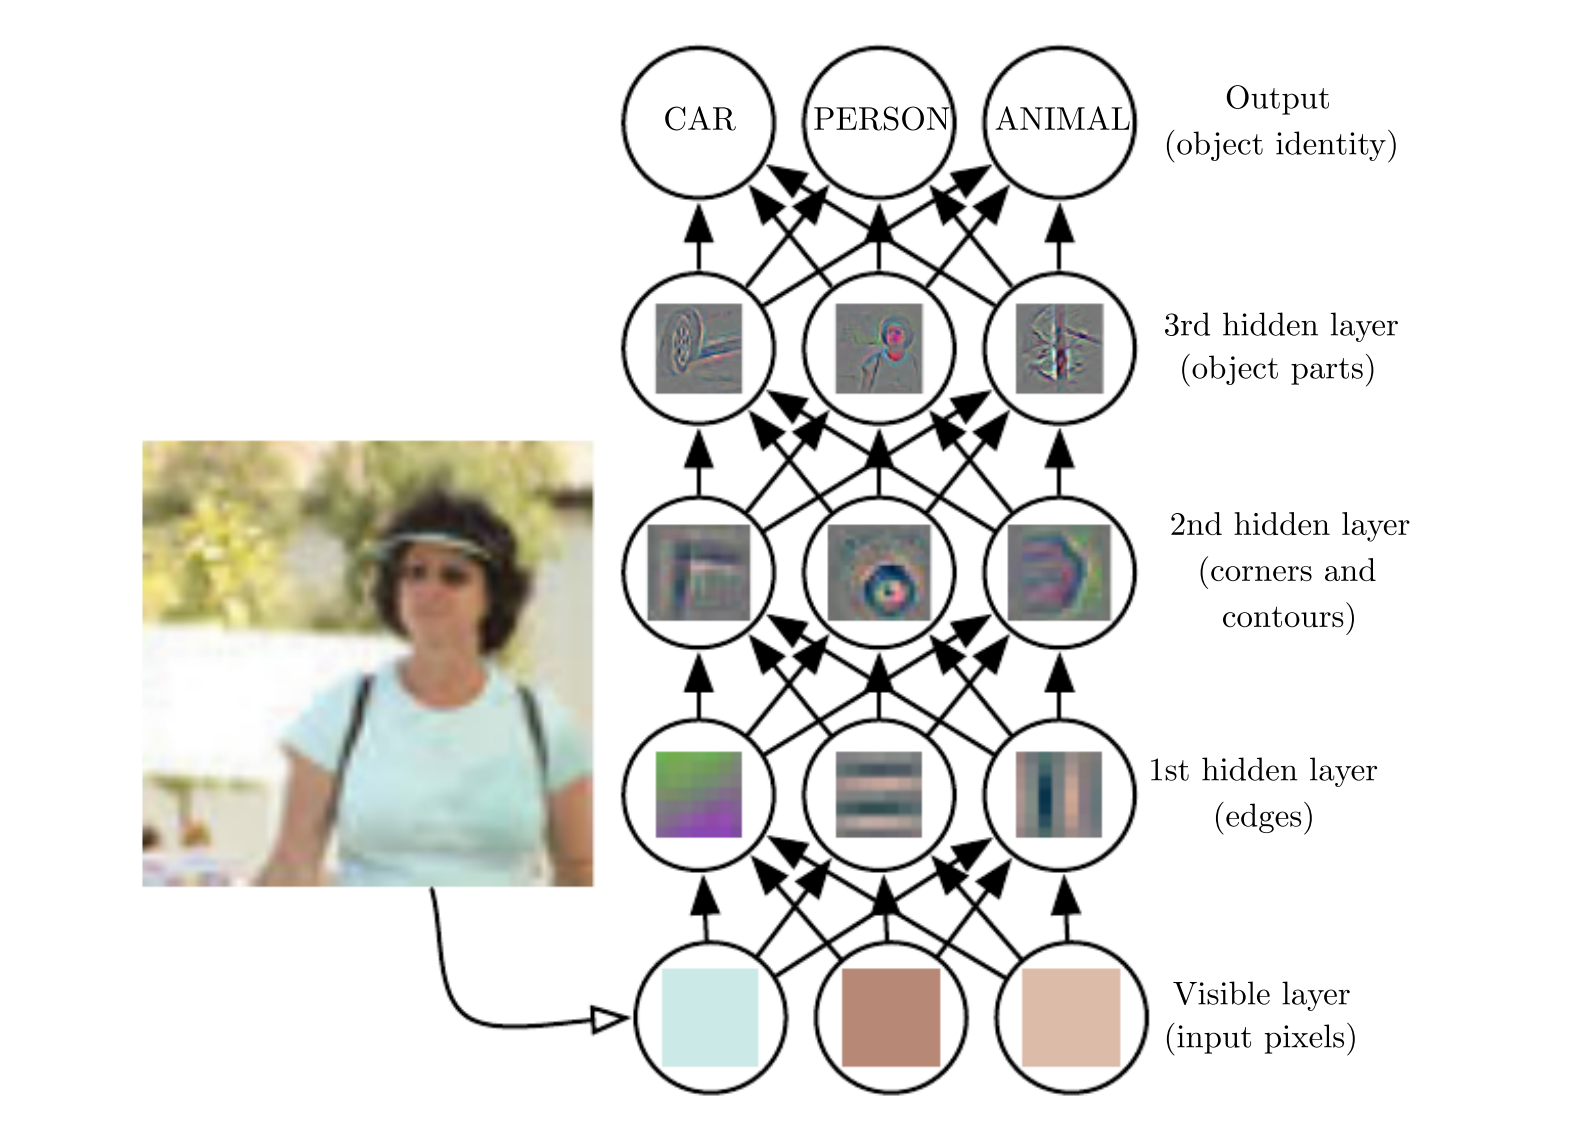
\includegraphics[width=12cm]{kapitel2/vision.png}
  \caption[Illustration eines Deep-Learning-Modells]{Illustration eines Deep-Learning-Modells aus \cite{IanGoodfellowYoshuaBengio2016} und \cite{Suah2017}: Ein Computer kann ohne weiteres das Bild in dieser Abbildung nicht erfassen, da es keine sensorischen Rohdaten verstehen kann. Das Bild in dieser Abbildung ist nur eine Sammlung von Pixelwerten. Die Funktionszuordnung von einem Satz von Pixeln zu einer Objektidentität ist sehr kompliziert.  Deep Learning löst diese Schwierigkeit, indem das gewünschte komplizierte \enquote{Mapping} in eine Reihe verschachtelter einfacher Mappings aufgeteilt wird, die jeweils durch eine andere Ebene des Modells beschrieben werden. Die Eingabe wird auf der \enquote{sichtbaren Ebene} (visible layer) dargestellt. Diese Schicht wird so genannt, weil sie die Variablen enthält, die wir beobachten können. Dann extrahieren eine Reihe \enquote{versteckter Ebenen} (hidden layer) zunehmend abstrakte Merkmale aus dem Bild. Diese Ebenen werden als \enquote{versteckt} bezeichnet, da ihre Werte nicht in den Daten angegeben sind. Stattdessen muss das Modell bestimmen, welche Konzepte zur Erklärung der Beziehungen in den beobachteten Daten nützlich sind. Angesichts der Pixel kann die erste Schicht Kanten nur leicht identifizieren, indem die Helligkeit benachbarter Pixel vergleicht. Angesichts der Beschreibung der Kanten durch die erste verborgene Ebene kann die zweite verborgene Ebene nach Ecken und erweiterten Konturen suchen. Angesichts der Beschreibung des Bildes durch die zweite verborgene Ebene in Bezug auf Ecken und Konturen kann die dritte verborgene Ebene ganze Teile bestimmter Objekte erkennen, indem bestimmte Konturen und Ecken gefunden werden. Schließlich kann diese Beschreibung des Bildes in Bezug auf die darin enthaltenen Objektteile verwendet werden, um die im Bild vorhandenen Objekte zu erkennen.}
  \label{Kap2:Vison}
\end{figure}

\section{Das Perzeptron}
Das Perzeptron kann ins deutsche mit dem Begriff der \enquote{Wahrnehmung} übersetzt werden. Das Perzeptron ist ein einfacher Algorithmus mit einem Eingabevektor $x$ mit $m$ Werten $(x_2, ..., x_m)$. Es wird oft wird als \enquote{Eingabe-Features} oder einfach als \enquote{Features} bezeichnet und zurückgegeben wird entweder eine $1$ \enquote{Ja} oder eine $0$ \enquote{Nein} (siehe Formel~\ref{Formel2_1}).

In Formel~\ref{Formel2_1}  ist $w$ ein Vektor welches das Gewicht darstellt, und $wx$ das Punktprodukt aus $\begin{array}{l}
    {\textstyle \sum ^{m}_{j=1}} w_{j} x_{j} \\
  \end{array}$, $b$ ist der Bias.
Aus $wx + b$ ist die Grenzhyperebene definiert, die die Position gemäß den $w$ und $b$ zugewiesenen Werten ändert.

\begin{equation}
  fx=\begin{cases}
    1 & wx+b >0   \\
    0 & ansonsten
  \end{cases}
  \label{Formel2_1}
\end{equation}

Mit anderen Worten, ist dies ein sehr einfacher, aber effektiver Algorithmus. Beispielsweise kann das Perzeptron bei drei Eingabemerkmalen  (Rot, Grün und Blau) unterscheiden, ob die Farbe weiß ist oder nicht. Es soll beachtet werden, dass das Perzeptron keine \enquote{Vielleicht}-Antwort ausdrücken kann. Es kann mit \enquote{Ja} (1) oder \enquote{Nein} (0) antworten. Das Perzeptron-Modell kann also benutzt werden, indem durch Anpassung von $w$ und $b$, das Modell \enquote{trainiert} wird.


\section{Mehrschichtiges Perzeptron}
In der Vergangenheit war \enquote{Perzeptron} der Name eines Modells mit einer einzigen linearen Schicht. Wenn es mehrere Schichten hat, wurde es daher als mehrschichtiges Perzeptron (Multi-layer perceptron / MLP) bezeichnet. Die Eingabe- und Ausgabeebene  ist von außen sichtbar, während alle anderen Ebenen in der Mitte ausgeblendet sind - daher der Name ausgeblendete Ebenen (hidden layers). In diesem Zusammenhang ist eine einzelne Schicht einfach eine lineare Funktion, und der MLP wird daher erhalten, indem mehrere einzelne Schichten nacheinander gestapelt werden (siehe Abbildung~\ref{Kap2:Multi}).

\begin{figure}[H]
  \centering
  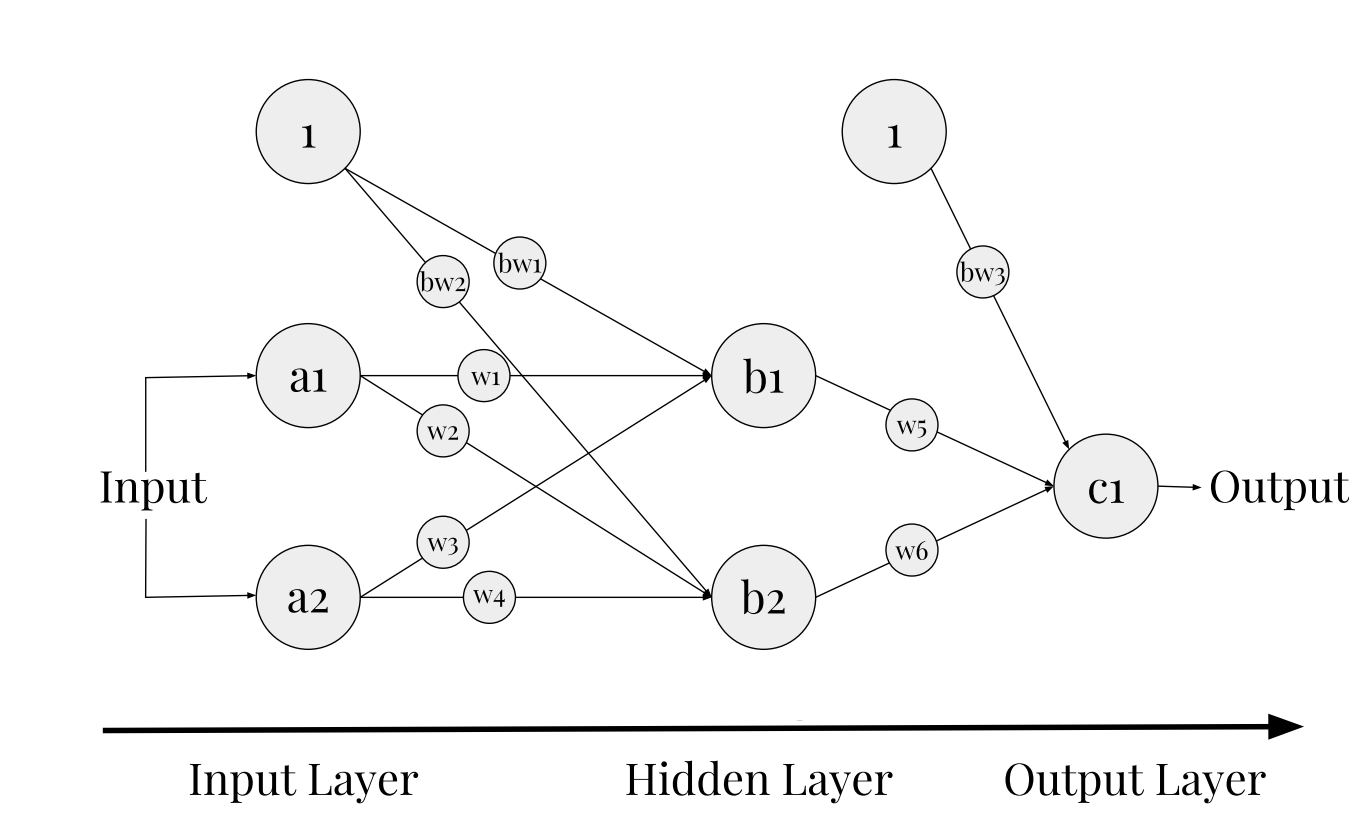
\includegraphics[width=12cm]{kapitel2/multilayer.png}
  \caption[Das mehrschichtige Perzeptron]{Ein Beispiel für ein mehrschichtiges Perzeptron in Anlehnung an \cite{Taylor2017}: Jeder Knoten in der ersten verborgenen Schicht empfängt eine Eingabe und \enquote{feuert} eine 0 oder 1 gemäß den Werten der zugehörigen linearen Funktion. Dann wird die Ausgabe der ersten verborgenen Schicht an die zweite Schicht übergeben, wo eine andere lineare Funktion angewendet wird, deren Ergebnisse an die endgültige Ausgabeschicht übergeben werden. Die letzte Schicht besteht nur aus einem einzelnen Neuron. Es ist interessant festzustellen, dass diese geschichtete Organisation vage der Organisation des menschlichen Sichtsystems ähnelt, wie zuvor besprochen.}
  \label{Kap2:Multi}
\end{figure}

Was sind die besten Entscheidungen für das Gewicht $w$ und den Bias $b$? Um diese Frage zu beantworten, wird nur ein einzelnes Neuron (ein einzelner Knoten) betrachtet.

Im Idealfall werden eine Reihe von Trainingsbeispielen bereitgestellt und der Computer muss das Gewicht $w$ und den Bias $b$ so einstellen, dass die in der Ausgabe erzeugten Fehler minimiert werden.

Um dies etwas konkreter zu machen, wird angenommen, dass es eine Reihe von Katzenbildern vorhanden sind und eine weitere separate Reihe von Bildern, die keine Katzen enthalten. Angenommen, jedes Neuron empfängt Eingaben vom Wert eines einzelnen Pixels in den Bildern. Während der Computer diese Bilder verarbeitet, möchten wir, dass unser Neuron seine Gewichte und seine Vorspannung so anpasst, dass immer weniger Bilder falsch erkannt werden.
Dieser Ansatz scheint sehr intuitiv zu sein, erfordert jedoch eine kleine Änderung der Gewichte (oder des Bias), um nur eine kleine Änderung der Ausgänge zu bewirken. Wenn wir einen großen Leistungssprung haben, können wir nicht progressiv lernen. Es wird gewünscht, wie ein \enquote{Kind} zu lernen, nach und nach. Das Perzeptron zeigt jedoch dieses \enquote{Stück für Stück}-Verhalten nicht. Ein Perzeptron gibt entweder eine 0 oder eine 1 zurück und das ist ein großer Sprung, der beim Lernen nicht hilft.


\section{Sigmoid-Neuron}
Das Verhalten des Perzeptron ist sehr  \enquote{uneben}, sodass ein \enquote{glatteres} nötig ist. Wir brauchen eine Funktion, die sich ohne Diskontinuität schrittweise von 0 auf 1 ändert. Mathematisch bedeutet dies, dass wir eine stetige Funktion benötigen, mit der wir die Ableitung berechnen können.

Dieses Problem kann überwunden werden, indem einen neuer Typ eines künstlichen Neurons eingeführt wird, der als Sigmoid-Neuron. Sigmoidneuronen ähneln Perzeptronen, sind jedoch so modifiziert, dass kleine Änderungen ihres Gewichts und ihres Bias nur eine geringe Änderung ihrer Leistung bewirken. Dies ist die entscheidende Tatsache, die es einem Netzwerk von Sigmoidneuronen ermöglicht, zu lernen \cite*[S. 8]{Nielsen}.

Genau wie ein Perzeptron hat das Sigmoid-Neuron die Eingaben $x_1, x_2, ...$, aber anstatt nur 0 oder 1 zu sein, können diese Eingänge auch beliebige Werte zwischen 0 und 1 annehmen. Also zum Beispiel 0,123 welches eine gültige Eingabe für ein Sigmoid-Neuron ist. Ebenso wie ein Perzeptron hat das Sigmoid-Neuron Gewichte für jede Eingabe, $w_1, w_2, ...$ und einen Bias, $b$. Die Ausgabe ist jedoch nicht 0 oder 1, stattdessen ist es $\sigma$, $(wx + b)$, wobei $\sigma$ als Sigmoidfunktion bezeichnet wird und durch Formel~\ref{Formel2_2} definiert ist.

\begin{equation} \label{Formel2_2}
  \sigma (z) = \frac{1}{1+e^{-z}}
\end{equation}


\section{Aktivierungsfunktionen}
Ohne eine Aktivierungsfunktion (auch als Nichtlinearität bezeichnet) würde die dichte Schicht (dense layer) nuraus zwei linearen Operationen bestehen - einem Punktprodukt und einer Addition: $Ausgabe = Punkt (w, Eingabe) + b$. Die Schicht konnte also nur lineare Transformationen (affine Transformationen) der Eingabedaten lernen. Um Zugang zu einem viel umfangreicheren Hypothesenraum zu erhalten, wird eine Nichtlinearitäts- oder Aktivierungsfunktion benötigt \cite*[S. 72]{Chollet2017}. Es gibt weitaus mehr Aktivierungsfunktionen, als die in die in diesem Abschnitt beschriebenen. Es sollen hier nur die gängigsten 3 vorgestellt werden.

\subsection{Sigmoid}
Die Sigmoidfunktion wurde bereits mit der Formel~\ref{Formel2_2} definiert und in der Abbildung~\ref{Kap2:Sigmoid_plot} dargestellt. Sie hat kleine Ausgangsänderungen im Bereich (0, 1), wenn der Eingang im Bereich $(-\infty, \infty)$ variiert. Mathematisch ist die Funktion stetig. Ein Neuron kann das Sigmoid zur Berechnung der nichtlinearen Funktion $\sigma(z = wx + b)$ verwenden.
Wenn $z = wx + b$ sehr groß und positiv ist, dann wird $e^z \rightarrow 0$ also $\sigma(z) \rightarrow 1$, während wenn $z = wx + b$ sehr groß und negativ ist dann wird $e^{-z} \rightarrow 0$ also $\sigma(z) \rightarrow 0$. Mit anderen Worten, ein Neuron mit Sigmoidaktivierung hat ein ähnliches Verhalten wie das Perzeptron, aber die Änderungen sind allmählich und Ausgabewerte wie 0,54321 oder 0,12345 sind vollkommen legitim. In diesem Sinne kann ein Sigmoid-Neuron \enquote{vielleicht} antworten \cite*[S. 10]{AntonioGuili;AmitaKapoor;SujitPal2019}.
\begin{figure}[H]
  \centering
  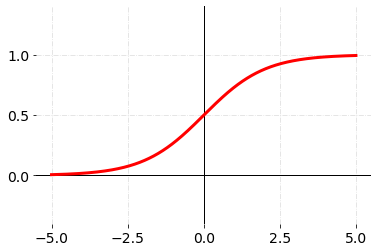
\includegraphics[width=8cm]{kapitel2/sig_plot.png}
  \caption[Darstellung der Sigmoid-Aktivierungsfunktion]{Darstellung der Sigmoid-Aktivierungsfunktion (eigene Darstellung)}
  \label{Kap2:Sigmoid_plot}
\end{figure}

\subsection{Tanh}
Die Tanh-Aktivierungsfunktion wird mit der Formel~\ref{Formel2_3} definiert. Sie hat ihre Ausgangsänderungen im Bereich (-1, 1). Sie hat eine Struktur, die der Sigmoid-Funktion sehr ähnlich ist. Der Vorteil gegenüber der Sigmoidfunktion besteht darin, dass ihre Ableitung steiler ist, was bedeutet, dass sie mehr Wert erhalten kann (vergleiche Abbildung~\ref{Kap2:Tanh_plot}).

\begin{equation} \label{Formel2_3}
  tanh(z) = \frac{e^{z}-e^{-z}}{e^{z}-e^{-z}}
\end{equation}

\begin{figure}[H]
  \centering
  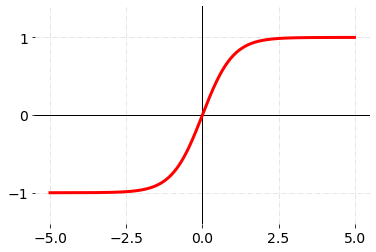
\includegraphics[width=8cm]{kapitel2/tanh_plot.png}
  \caption[Darstellung der Tanh-Aktivierungsfunktion]{Darstellung der Tanh-Aktivierungsfunktion (eigene Darstellung)}
  \label{Kap2:Tanh_plot}
\end{figure}

\subsection{ReLu}
Vor kurzem wurde eine sehr einfache Funktion namens ReLU (REctified Linear Unit) sehr beliebt, da sie dazu beiträgt, einige bei Sigmoiden beobachtete Optimierungsprobleme zu lösen \cite*[S. 11]{AntonioGuili;AmitaKapoor;SujitPal2019}. Eine ReLU wird relativ einfach in und wird in der Formel~\ref{Formel2_4} definiert. Wie in Abbildung~\ref{Kap2:ReLu_plot} zu sehen, ist die Funktion für negative Werte Null und wächst für positive Werte linear. Die ReLU ist auch sehr einfach zu implementieren (im Allgemeinen reichen drei Anweisungen aus), während das Sigmoid einige Größenordnungen mehr benötigt.

\begin{equation} \label{Formel2_4}
  f( x) \ =\ \begin{cases}
    0 & \textrm{\textit{für}}\ x < \ 0   \\
    x & \textrm{\textit{für}}\ x\geq \ 0
  \end{cases}
\end{equation}

\begin{figure}[H]
  \centering
  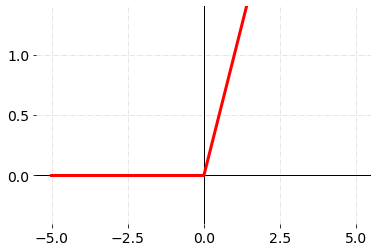
\includegraphics[width=8cm]{kapitel2/relu_plot.png}
  \caption[Darstellung der ReLu-Aktivierungsfunktion]{Darstellung der ReLu-Aktivierungsfunktion (eigene Darstellung)}
  \label{Kap2:ReLu_plot}
\end{figure}




\section{Verlustfunktion und Kreuzentropie}
Innerhalb eines neuronalen Netzwerks wandelt eine Verlustfunktion alle möglichen Fehler, in eine Zahl um, die den Gesamtfehler des Netzwerks darstellt. Im Wesentlichen ist es ein Maß dafür, wie falsch ein Netzwerk ist. Auf einer technischeren Ebene werden ein Ereignis oder Werte einer oder mehrerer Variablen einer reellen Zahl zugeordnet. Diese reelle Zahl stellt  den \enquote{Verlust} oder die \enquote{Kosten} dar, die mit dem Ereignis oder den Werten verbunden sind \cite*[S. 41]{Taylor2017}.

\subsection{Mittlere quadratische Abweichung}
Wie der Name sagt, wird mit der mittleren quadratischen Abweichung (MSE), der Verlust berechnet, indem der Mittelwert der quadratischen Differenzen zwischen tatsächlichen Ziel- und vorhergesagten Werten genommen wird. Sie wird in Formel~\ref{Formel2_5} definiert.

\begin{equation} \label{Formel2_5}
  MSE\ =\frac{1}{n}{\displaystyle \sum ^{n}_{i=1}( d-y)^2}
\end{equation}

Diese Funktion ist der Durchschnitt aller Fehler, die in jeder Vorhersage gemacht wurden. Wenn eine Vorhersage weit vom wahren Wert entfernt ist, wird dieser Abstand durch die \enquote{Quadrierungsoperation} deutlicher. Außerdem kann das Quadrat den Fehler addieren, unabhängig davon, ob ein bestimmter Wert positiv oder negativ ist \cite*[17]{AntonioGuili;AmitaKapoor;SujitPal2019}.

Grundsätzlich kann diese Verlustfunktion verwendet werden, wenn die Ausgabe eine reelle Zahl ist. Die MSE-Verlustfunktion wird meistens für Regressionsaufgaben verwendet.

\subsection{Binäre Kreuzentropie}
\subsection{Kategoriale Kreuzentropie}


% \section{Formelsatz}

% Eine Formel gefällig? Mitten im Text $a_2 = \sqrt{x^3}$ oder als eigener Absatz (siehe Formel~\ref{Formel}):




% Das Aufkommen von Online-Nachrichtenagenturen und die Explosion der Anzahl der Benutzer, die Nachrichten mit diesem Medium konsumieren, haben dazu geführt, dass mehrere Webseiten miteinander konkurrieren, um die Aufmerksamkeit der Benutzer zu erregen. Dies hat dazu geführt, dass Verkaufsstellen kreative Wege geschaffen haben, um Leser auf ihre Website zu locken. Eine der am häufigsten verwendeten Techniken ist die Verwendung von Clickbait-Überschriften. Diese Überschriften wurden speziell dafür entwickelt, um das Interesse des Lesers an dem zu wecken, was versprochen wird. Wenn auf den Artikel geklickt wird jedoch, liefert dieser Artikel normalerweise nicht den Inhalt, den der Leser Ursprüngich gesucht hat. In den Abbildungen \ref{Kap2:ClickBait} und \ref{Kap2:News}\footnote{Entnommen aus: https://github.com/MichaelGoodale/Clickbait-Classifier} wird der Unterschied zwischen Clickbaits und \enquote{normalen} Nachrichten aufgezeigt.

% \begin{figure}
%   \centering
%   \includegraphics[width=12cm]{kapitel2/clickbait.png}
%   \caption[Beispiel von Clickbait]{Beispiel von Clickbait}
%   \label{Kap2:ClickBait}
% \end{figure}


% \begin{figure}[ht]
%   \centering
%   \includegraphics[width=12cm]{kapitel2/news.png}
%   \caption[Beispiel von \enquote{normalen} Nachrichten]{Beispiel von \enquote{normalen} Nachrichten}
%   \label{Kap2:News}
% \end{figure}


% \section{Lösungsansatz}
% Textklassifizierung ist eine gängige Art, wie man \enquote{gute} von \enquote{bösen} Texten unterscheiden kann. Es ist allerdingt nicht praktisch ein großes Sprachmodell wie GPT-3 Browserkompatible zu machen. Erstens ist es völlig \enquote{overkill} für ein solches Problem ein Sprachmodell zu benutzen und zweitens passen diese großen Modelle nicht in den Browser, da die Ladezeit nicht praktisch ist.

% Mit dieser Arbeit möchte ich ein Modell erstellen, um Clickbait Überschriften zu erkennen. Es wäre Hilfreich, wenn es ein Dienst gibt, welches eine Überschrift liest und dem Benutzer vorhersagt, ob es sich um Clickbait handelt oder nicht. So kann der Nutzer seine Zeit sparen und muss nicht auf die Seite gehen. Das Hauptprodukt ist dabei dieser Dienst, welches ganz einfach in jede HTML-Seite importiert werden kann. Dieser Dienst muss klein und schnell und gute dabei möglichst Ergebnisse liefern.

% \section{Aufbau der Arbeit}


% Im Abschnitt 2.6 Grobgliederung befindet sich eine mögliche Gliederung für diese Arbeit, auf die ich verweisen möchte. Zunächst wird in den Kapiteln 2 und 3 eine theoretische Grundlage geschaffen. Diese Kapitel beschäftigen sich mit Deep Learning und den mathematisch/statistschischen Erklärungen. Kapitel 3 orientiert sich eher mit NLP und insbesondere mit Worteinbettungen und wie moderne Computer die natürliche Sprache verstehen. Kapitel 4 soll den aktuellen Forschungsstand mit meiner Arbeit vergleichen. Es sollen verwandte Lösungsansätze kategorisch analysiert werden.

% Um mit dem eigentlichen Kern anzufangen, benötigt diese Arbeit an Daten. In Kapitel 5 wird gezeigt wie mittelt Webscraping. Dieser Datensatz wird händisch gelabelt und besteht aus einem Titel und einer Klasse. Die erste erste hälfte des Datensatzes wird aus Wikinews\footnote{https://de.wikinews.org/wiki/Hauptseite} geladen. Wikinews hat einen API-Zugang wodurch Nachrichten, welche nicht Clickbait sind in den Datensatz gebracht werden können. Ich habe dafür bereits mehr als 10.000 Nachrichten-Titel in eine Datenbank geladen. Die zweite hälfte des Datensatzes wird mittels Webseiten mit Scrapy\footnote{ https://scrapy.org/} gescraped. Die ersten 1.000 Titel sind bereits in die Datenbank\footnote{https://github.com/youurt/klickkoeder/blob/main/klickscraper/klickscraper.db} geladen worden.

% Nachdem ausreichend Daten geladen werden, ist geplant diese Daten zu laben. Damit später keine Verzerrungen bei den Daten entstehen, plane ich noch eine weitere Person zum Unterstützen beim Labeln mit in die Arbeit zu nehmen. Dieses wird mit dem Betreuer der Arbeit noch abgeklärt werden müssen. Der restliche Teil dieses Kapitels beschäftigt sich mit der Analyse der Daten um bestimmte Muster zu erkennen und die Daten in ein passendes Format zu bringen.

% Ich werde ein Modell in TensorFlow.js entwickeln. Dieses Modell soll möglichst klein sein und schnell sein. Um mit TensorFlow.js arbeiten zu können muss der Text in Vektoren umgewandelt werden.

% Mit einem Versuchsaufbau soll das Modell getestet und analysiert werden. Schließlich soll das Modell in die Browser-Umgebung gebracht und mittels eines minimalistischen React Frontends angeboten werden.

% \begin{figure}[ht]
%   \centering
%   \includegraphics[width=12cm]{kapitel2/beispiel.png}
%   \caption[Beispiel einer Systemarchitektur]{Beispiel einer Systemarchitektur entnommen aus \cite{cho2019shop}. Der Client bekommt beim laden der Seite, neben dem HTML, CSS und dem JavaScript, welches für das Frontend nötig ist, ein weiteres Script, welches die TensorFlow.js API bereitstellt. Die Berechnung findet im Browser, beim Client statt, wo auch das Modell sich befindet.}
%   \label{Kap2:SystemArchitektur}
% \end{figure}

% \section{Wissenschaftlicher Beitrag}
% \begin{itemize}
%   \item Den Stand der Technik in Bezug auf Deep Learning und Worteinbettungen zeigen
%   \item Erstellung und labeln eines Datensatzes für deutsche Clickbaits
%   \item Implementierung eines NLP-Problemes im Browser ohne zusätzliche Software oder Plugins, mit TensorFlow.js
%   \item Optimierung des Browsers für Deep Learning
%   \item Auswahl des optimalen Modells und der Trainingsmethode
%   \item Produktion eines Dienstes, um Clickbait Nachrichten vorzubeugen
% \end{itemize}

% \section{Einstiegsliteratur}

% \begin{itemize}
%   \item \cite{Kaur2020a}
%   \item \cite{Chavan2019}
%   \item \cite{vorakitphan2018clickbait}
%   \item \cite{Anand2017}
%   \item \cite{gairola2017neural}
%   \item \cite{kumar2018identifying}
%   \item \cite{glenski2017fishing}
%   \item \cite{chawda2019novel}
%   \item \cite{seopredicting}
%   \item \cite{cho2019shop}
%   \item \cite{roberts2018magenta}
%   \item \cite{aggarwal2012survey}
%   \item \cite{kowsari2019text}
%   \item \cite{korde2012text}
%   \item \cite{altinel2018semantic}
%   \item \cite{nordberg2020crucial}
%   \item \cite{raamkumar2020use}
%   \item \cite{rivera2020identifying}
%   \item \cite{nguyen2020real}
%   \item \cite{zhang2015character}
%   \item \cite{kiranyaz20191d}
%   \item \cite{severyn2015unitn}
%   \item \cite{severyn2015twitter}
%   \item \cite{zhao2019speech}
%   \item \cite{eren2019generic}
% \end{itemize}

% \section{Grobgliederung}
% \renewcommand{\labelenumii}{\theenumii}
% \renewcommand{\theenumii}{\theenumi.\arabic{enumii}.}

% \begin{enumerate}

%   \item Einleitung
%         \begin{enumerate}
%           \item Motivation
%           \item Wissenschaftlicher Beitrag
%           \item Struktur der Arbeit
%         \end{enumerate}

%   \item Neuronale Netze
%         \begin{enumerate}
%           \item Einleitung
%           \item Arten des Neuronalen Lernens
%           \item Netzwerkparameter und Hyperparameter
%           \item Aktivierungsfunktionen
%           \item Verlustfunktion
%           \item Optimizer
%           \item Epochen
%           \item TensorFlow.js
%           \item Schluss
%         \end{enumerate}

%   \item Die natürliche Sprache
%         \begin{enumerate}
%           \item Einleitung
%           \item Vektorisierung des Textes durch Encoding
%           \item Worteinbettungen
%           \item 1d CNN
%           \item Schluss
%         \end{enumerate}

%   \item Aktueller Forschungsstand
%         \begin{enumerate}
%           \item Einleitung
%           \item Clickbaits und Deep Learning Ansätze
%           \item TensorFlow.js
%           \item Worteinbettungen
%         \end{enumerate}

%   \item Korpuskonstruktion und Analyse
%         \begin{enumerate}
%           \item Einleitung
%           \item Rohdatenerhebung mittels Webscraping
%           \item Das labeln der Daten
%           \item Explorative Datenanalyse
%           \item Vorverarbeitung der Daten
%           \item Schluss
%         \end{enumerate}

%   \item Methodik
%         \begin{enumerate}
%           \item Einleitung
%           \item Die Systemarchitektur
%           \item JavaScript
%           \item Modelling
%           \item Einbettung in das Frontend
%           \item Schluss
%         \end{enumerate}

%   \item Versuchsaufbau und Diskussion der Ergebnisse
%         \begin{enumerate}
%           \item Einleitung
%           \item Anpassung der Netzwerkparameter und Hyperparameter
%           \item Leistungsmessungen
%           \item Vergleich und Darstellung der Ergebnisse
%           \item Schluss
%         \end{enumerate}

%   \item Schluss
%         \begin{enumerate}
%           \item Fazit zum Forschungsbeitrag
%           \item Abschließende Gedanken
%           \item Zukunft der Arbeit
%         \end{enumerate}
% \end{enumerate}




% \section{Hervorhebungen}
% \label{Einleitung:Textauszeichnungen}

% Achten Sie bitte auf die grundlegenden Regeln der Typographie\index{Typographie}\footnote{Ein Ratgeber in allen Detailfragen ist \cite{Forssman2002}.}, wenn Sie Ihren Text schreiben. Hierzu gehören z.\,B. die Verwendung der richtigen "`Anführungszeichen"' und der Unterschied zwischen Binde- (-), Gedankenstrich (--) und langem Strich (---). Sie erhalten den Bindestrich in \LaTeX{} mit \verb+-+, den Gedankenstrich mit \verb+--+ und den langen Strich mit \verb+---+.

% Wenn Sie Text hervorheben wollen, dann setzten Sie ihn mit \verb+\textit+ \textit{kursiv} (Italic) und nicht \textbf{fett} (Bold). Fettdruck ist Überschriften vorbehalten; im Fließtext stört er den Lesefluss. Das \underline{Unterstreichen} von Fließtext ist im gesamten Dokument tabu und kann maximal bei Pseudo"=Code vorkommen.\index{Hervorhebungen}


% \section{Anführungszeichen}

% Deutsche Anführungszeichen werden mit \verb+"`+ und \verb+"'+ erzeugt: "`dieser Text steht in \glq Anführungszeichen\grq; alles klar?"'. Englische Anführungszeichen hingegen mit \verb+``+ und \verb+''+: ``this is an `English' quotation''. Beachten Sie, dass Sie in Zitaten immer die zur Sprache passenden Anführungszeichen verwenden. Die Verwendung von \verb+"+ ist für Anführungszeichen immer falsch und führt bei \LaTeX{} zu seltsamen "Effekten".

% Um sich diesen Ärger zu sparen, biete sich die Verwendung des Paketes \textit{csquotes} und des Kommandos \verb+\enquote+ an. Hierdurch werden die Anführungszeichen korrekt für die eingestellte Sprache gesetzt und Sie müssen sich \enquote{keine Sorgen mehr über die \enquote{Anführungszeichen} machen}.


% \section{Abkürzungen}
% \index{Abkürzungen}
% \index{Abbreviation|see{Abkürzungen}}

% Eine \ac{ABK} (\verb+\ac{ABK}+) wird bei der ersten Verwendung ausgeschrieben. Danach nicht mehr: \ac{ABK}. Man kann allerdings mit \verb+\acl+ die Langform explizit anfordern (\acl{ABK}) oder mit \verb+\acs+ die Kurzform (\acs{ABK}) oder mit \verb+\acf+ auch noch einmal die Definition (\acf{ABK}).

% Beachten Sie, dass bei Abkürzungen, die für zwei Wörter stehen, ein kleines Leerzeichen nach dem Punkt kommt: z.\,B. bzw. \zb{} und d.\,h. bzw. \dahe{}. Das Template bietet hierfür die beiden Makros \verb+\zb{}+ und \verb+\dahe{}+.


% \section{Querverweise}

% Querverweise auf eine Kapitelnummer macht man im Text mit \verb+\ref+ (Kapitel~\ref{Einleitung:Textauszeichnungen}) und auf eine bestimmte Seite mit \verb+\pageref+ (Seite~\pageref{Einleitung:Textauszeichnungen}). Man kann auch den Befehl \verb+\autoref+ benutzen, der automatisch die Art des referenzierten Elements bestimmt (\zb{} \autoref{Einleitung:Textauszeichnungen} oder \autoref{Kap2:Kopplungsformen}).


% \section{Fußnoten}

% Fußnoten werden einfach mit in den Text geschrieben und zwar genau an die Stelle\footnote{An der die Fußnote auftauchen soll}. Hierzu dient der Befehl \verb+\footnote{Text}+.


% \section{Tabellen}

% Tabellen werden normalerweise ohne vertikale Striche gesetzt, sondern die Spalten werden durch einen entsprechenden Abstand voneinander getrennt.\footnote{Siehe \cite[S. 89]{Willberg1999}.} Zum Einsatz kommen ausschließlich horizontale Linien (siehe Tabelle~\ref{Kap2:Kopplungsformen}).

% \begin{table}[h]
%   \caption{Ebenen der Kopplung und Beispiele für enge und lose Kopplung}
%   \label{Kap2:Kopplungsformen}
%   \renewcommand{\arraystretch}{1.2}
%   \centering
%   \sffamily
%   \begin{footnotesize}
%     \begin{tabular}{l l l}
%     \toprule
%     \textbf{Form der Kopplung} & \textbf{enge Kopplung} & \textbf{lose Kopplung}\\
%     \midrule
%     Physikalische Verbindung	&	Punkt-zu-Punkt	& 	über Vermittler\\
%     Kommunikationsstil	&	synchron		&	asynchron\\
%     Datenmodell	&	komplexe gemeinsame Typen	&	nur einfache gemeinsame Typen\\
%     Bindung	&	statisch		&	dynamisch\\
%     \bottomrule
%     \end{tabular}
%   \end{footnotesize}
%   \rmfamily
% \end{table}

% Eine Tabelle fließt genauso, wie auch Bilder durch den Text. Siehe Tabelle~\ref{Kap2:Kopplungsformen}.

% Manchmal möchte man Tabellen, in denen der Text in der Tabellenspalte umbricht. Hierzu dient die Umgebung \texttt{tabularx}, wobei \texttt{L} eine Spalte mit Flattersatz und \texttt{X} eine mit Blocksatz definiert. Die Breite der Tabelle kann über den Faktor vor \verb+\textwidth+ angegeben werden.

% \begin{table}[h]
%   \caption{Teildisziplinen der Informatik}
%   \label{Kap2:Teildisziplinen}
%   \renewcommand{\arraystretch}{1.2}
%   \centering
%   \sffamily
%   \begin{footnotesize}
%     \begin{tabularx}{0.9\textwidth}{l X L}
%       \toprule
%       \textbf{Gebiet} & \textbf{Definition} & \textbf{Beispiel}\\
%       \midrule
%       \emph{Praktische Informatik} & Informatik-Disziplinen, welche sich vorwiegend mit der Entwicklung und Anwendung der Software-Komponenten befassen & Programmentwicklung, Compilerbau; im Aufbau von z.B. Informationssystemen und Netzwerken ergeben sich Überlappungen mit der technischen Informatik \\
%       \emph{Technische Informatik} & Informatik-Disziplinen, welche sich vorwiegend mit der Entwicklung und Anwendung der Hardware-Komponenten befassen & Digitaltechnik, Mikroprozessortechnik \\
%       \emph{Theoretische Informatik} & Informatik-Disziplinen, welche sich mit der Entwicklung von Theorien und Modellen der Informatik befassen und dabei viel Substanz aus der Mathematik konsumieren & Relationenmodell, Objekt-Paradigmen, Komplexitätstheorie, Kalküle \\
%       \emph{Angewandte Informatik} & Informatik als instrumentale Wissenschaft & Rechtsinformatik, Wirtschaftsinformatik, Geoinformatik \\
%       \bottomrule
%     \end{tabularx}
%   \end{footnotesize}
%   \rmfamily
% \end{table}


% \section{Harveyballs}

% \begin{quote}
%     Harvey Balls sind kreisförmige Ideogramme, die dazu dienen, qualitative Daten anschaulich zu machen. Sie werden in Vergleichstabellen verwendet, um anzuzeigen, inwieweit ein Untersuchungsobjekt sich mit definierten Vergleichskriterien deckt. \parencite{Wikipedia_HarveyBalls}
% \end{quote}

% \begin{table}[h]
%   \caption{Beispiel für Harvey Balls}
%   \label{tab:harveyexample}
%   \centering
%   \begin{tabular}{lccc}
%     \toprule
%     & Ansatz 1 & Ansatz 2 & Ansatz 3\\
%     \midrule
%     Eigenschaft 1	& \harveyBallNone & \harveyBallQuarter & \harveyBallHalf \\
%     Eigenschaft 2	& \harveyBallHalf & \harveyBallThreeQuarter & \harveyBallFull \\
%     Eigenschaft 3	& \harveyBallFull & \harveyBallThreeQuarter & \harveyBallQuarter\\
%     \bottomrule
%   \end{tabular}
% \end{table}


% \section{Aufzählungen}

% Aufzählungen sind toll.

% \begin{itemize}
%   \item Ein wichtiger Punkt
%   \item Noch ein wichtiger Punkt
%   \item Ein Punkt mit Unterpunkten
%     \begin{itemize}
%       \item Unterpunkt 1
%       \item Unterpunkt 2
%     \end{itemize}
%   \item Ein abschließender Punkt ohne Unterpunkte
% \end{itemize}


% Aufzählungen mit laufenden Nummern sind auch toll.

% \begin{enumerate}
%   \item Ein wichtiger Punkt
%   \item Noch ein wichtiger Punkt
%   \item Ein Punkt mit Unterpunkten
%     \begin{enumerate}
%       \item Unterpunkt 1
%       \item Unterpunkt 2
%     \end{enumerate}
%   \item Ein abschließender Punkt ohne Unterpunkte
% \end{enumerate}
 % Externe Datei einbinden
\chapter{Die Natürliche Sprache}


Die \textbf{Verarbeitung natürlicher Sprache} (NLP) ist ein theoretisch motivierter Bereich von Computertechniken, zum Analysieren und Darstellen natürlich vorkommender Texte auf einer oder mehreren Ebenen der Sprachanalyse, um eine menschenähnliche Sprachverarbeitung für eine Reihe von Aufgaben oder Anwendungen zu erreichen \cite*{Liddy}.

Der Umgang mit Textdaten ist problematisch, da unsere Computer, Skripte und Modelle für maschinelles Lernen, keinen Text im menschlichen Sinne lesen und verstehen können. Wörter können viele verschiedene Assoziationen aufrufen, diese sprachlichen Assoziationen sind das Ergebnis recht komplexer neurologischer Berechnungen. ML-Modelle sind haben dieses vorgefertigte Verständnis der Wortbedeutung nicht.


% regular expressions
% tokenize
% part of speech tagging
% ngrams

\section{Tokenisieren und Extrahieren durch Reguläre Ausdrücke}
Das Segmentieren eines Textes in seine Einheiten ist die erste Voraussetzung für dessen Weiterverarbeitung. In der Informatik können einzelne Wörter bzw. Tokens durch Leerzeichen voneinander abgetrennt werden.

Reguläre Ausdrücke können die Tokenisierung verbessern. Reguläre Ausdrücke sind eine Sprache zur Angabe von Textsuchzeichenfolgen. Diese praktische Sprache wird in allen Computersprachen, Textverarbeitungs- und Textverarbeitungswerkzeugen verwendet. Formal ist ein regulärer Ausdruck eine algebraische Notation zur Charakterisierung einer Reihe von Zeichenfolgen. Sie sind besonders nützlich für die Suche in Texten, wenn ein Muster gesucht wird und ein Korpus von Texten durchsucht werden muss. Eine Suchfunktion für reguläre Ausdrücke durchsucht den Korpus und gibt alle Texte zurück, die dem Muster entsprechen. Der Korpus kann ein einzelnes Dokument oder eine Sammlung sein \cite*[3]{Jurafskya}. Reguläre Ausdrücke sind also bestimmte Regeln die Muster in einem Text erkennen lassen. Neben der Tokenisierung können sie auch für das extrahieren von Informationen aus Textsequenzen verwendet werden, siehe Listing~\ref{Regex}.


\begin{lstlisting}[language=Python,caption=Das extrahieren der Zahlen aus einer URL]
>>> import re
>>> url = "http://www.example.com/this-2-me-4/123456-subj"
>>> print(re.search("/([0-9]+)-", url).group(1))

123456
\end{lstlisting}\label{Regex}
\section{N-Gramm}

Sprachmodelle sind Wortfolgen zu denen Wahrscheinlichkeiten zugewiesen wurden. Das einfachste Sprachmodell ist das N-Gramm Sprachmodell. Es ist eine Folge von N Wörtern (ein 2-Gramm oder Bigramm ist eine Folge von zwei Wörtern usw.). N-Gramm wird meistens dafür verwendet, um das nächste Wort in aus einer Sequenz vorherzusagen \cite*[31]{Jurafskya}. Angenommen ein Korpus besteht aus folgenden 4 Sätzen:

\begin{enumerate}
    \item Es regnet in Berlin.
    \item Es regnet in Köln und es ist 10 Grad.
    \item Es regnet und hagelt in ganz Deutschland.
    \item In Deutschland herrscht Regen.
\end{enumerate}

Um die Wahrscheinlichkeit \textit{P (regnet | in)} herauszufinden, wird die Anzahl des Wortes \enquote{regnet} im Korpus gezählt. Es wird gezählt, wie oft \enquote{regnet} und \enquote{in} zusammen vorkommen (2 Mal) und dieses wird dividiert durch 3, da \enquote{regnet} insgesamt 3 Mal im Korpus vorkommt. Das Bigramm \enquote{regnet in} hat also eine Wahrscheinlichkeit von 2/3.

\section{Part-of-Speech Tagging}
Part-of-Speech Tagging ist der Prozess des Zuweisens einer Tags zu jedem Wort in einem Eingabetext. Die Eingabe in einen Kennzeichnungsalgorithmus ist eine Folge von tokenisierten Wörtern und einem Tag-Satz, und die Ausgabe ist eine Folge von Tags, eines pro Token \cite*[148]{Jurafskya}. Je nach Sprache gibt es verschiedene Tagger, für das Deutsche gibt es das Stuttgart-Tübingen-Tagset\cite*{tagger}, einige Tags können aus der Tabelle~\ref{STTS} entnommen werden. Die Tagger wurden ursprünglich manuell erfasst und in heutiger Zeit durch das Maschinelle Lernen automatisiert.



\begin{table}[h]
    \caption{Beispiele aus dem Stuttgart-Tübingen-Tagset}
    \label{STTS}
    \renewcommand{\arraystretch}{1.2}
    \centering
    \sffamily
    \begin{footnotesize}
        \begin{tabular}{l l l}
            \toprule
            \textbf{POS} & \textbf{Beschreibung}                  & \textbf{Beispiel}                                  \\
            \midrule
            ADJA         & attributives Adjektiv                  & das \textit{große} Haus                            \\
            ADJD         & adverbiales oder prädikatives Adjektiv & er fährt \textit{schnell}, er ist \textit{schnell} \\
            ADV          & Adverb                                 & \textit{schon}, \textit{bald}, doch                \\
            NE           & Eigennamen                             & \textit{Hans}, \textit{Hamburg}, \textit{HSV}      \\
            NN           & normales Nomen                         & \textit{Tisch}, \textit{Herr}, das \textit{Reisen} \\
            VVFIN        & finites Verb, voll                     & du \textit{gehst}, wir \textit{kommen} an          \\
            \bottomrule
        \end{tabular}
    \end{footnotesize}
    \rmfamily
\end{table}




\section{Wie können Deep Learning Modelle die Natürliche Sprache lernen?}

Die verborgenen Schichten eines mehrschichtigen neuronalen Netzwerks lernen, die Eingaben des Netzwerks so darzustellen, dass die Zielausgaben leicht vorhergesagt werden können. Dies wird gut demonstriert, indem ein mehrschichtiges neuronales Netzwerk trainiert wird, um das nächste Wort in einer Sequenz aus einem lokalen Kontext früherer Wörter vorherzusagen \cite*{Bengio2003}. Jedes Wort im Kontext wird dem Netzwerk als Eins-aus-N-Vektor dargestellt, dh eine Komponente hat den Wert 1 und der Rest ist 0, dieses Verfahren wird auch als \textit{One-Hot-Encoding} bezeichnet. In einem \textit{Sprachmodell} lernen die anderen Schichten des Netzwerks, die Eingangswortvektoren in einen Ausgangswortvektor für das vorhergesagte nächste Wort umzuwandeln, welches verwendet werden kann, um die Wahrscheinlichkeit vorherzusagen, dass ein Wort im Vokabular als nächstes erscheinen wird \cite*{Lecun2015}. Das Netzwerk lernt \textbf{Wortvektoren}, die viele aktive Komponenten enthalten, von denen jede als separates Merkmal des Wortes interpretiert werden kann. Dieses Vorgehen wurde erstmals im Zusammenhang mit dem Lernen verteilter Darstellungen für Symbole demonstriert \cite*{Rumelhart1986}. Die semantischen Merkmale waren in der Eingabe nicht explizit vorhanden. Das Lernverfahren wurde als eine gute Möglichkeit entdeckt, die strukturierten Beziehungen zwischen den Eingabe- und Ausgabesymbolen in mehrere \enquote{Mikroregeln} zu zerlegen. Das Lernen von Wortvektoren hat sich auch als sehr gut erwiesen, wenn die Wortsequenzen aus einem großen Korpus von echtem Text stammen und die einzelnen Mikroregeln unzuverlässig sind \cite*{Bengio2003}.


\begin{figure}[H]
    \centering
    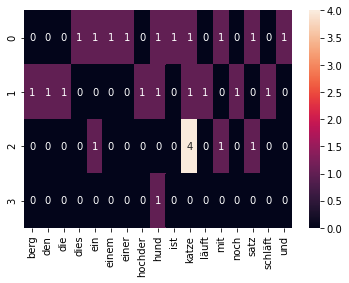
\includegraphics[width=8cm]{kapitel3/onhot.png}
    \caption[One-Hot-Codierung als Eingabematrix]{Die Grafik zeigt wie ein Beispielkorpus welches aus 5 Sätzen besteht, in einer Matrix dargestellt werden kann. Je nach Häufigkeit wird jedes Wort im Wortschaft entsprechend den Sätzen im Korpus abgebildet. Der Korpus besteht aus 5 Sätzen (\enquote{Dies ist ein Satz mit einer Katze und einem Hund.}, \enquote{Die Katze läuft den Berg hoch.}, \enquote{Der Hund schläft noch.}, \enquote{Ein Satz mit Katze Katze Katze Katze.} und \enquote{Ein Hund.}) (eigene Darstellung).}
    \label{OneHotGrafik}
\end{figure}

Die numerischen Werte sollten so viel wie möglich von der sprachlichen Bedeutung eines Wortes erfassen. Eine gut ausgewählte, informative Eingabedarstellung kann einen massiven Einfluss auf die Gesamtleistung des Modells haben. \textbf{Worteinbettungen} sind der vorherrschende Ansatz für dieses Problem und so weit verbreitet, dass ihre Verwendung praktisch in jedem NLP-Projekt angenommen wird. Unabhängig davon, ob Sie ein Projekt in den Bereichen Textklassifizierung, Sentimentanalyse oder maschinelle Übersetzung starten \cite*{Lecun2015}.


\section{Worteinbettungen}
Vektoren zur Darstellung von Wörtern werden im Allgemeinen als Einbettungen bezeichnet, da das Wort in einen bestimmten Vektorraum eingebettet wird \cite*[99]{Jurafskya}.

\begin{figure}[H]
    \centering
    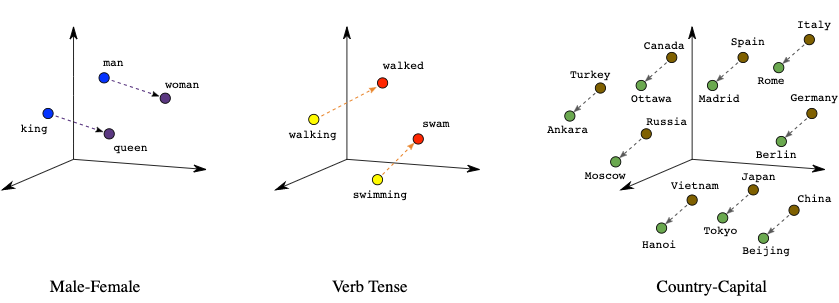
\includegraphics[width=14cm]{kapitel3/wordem.png}
    \caption[Worteinbettungen erzeugen Analogien zwischen Wörtern]{Durch Worteinbettungen können interessante Analogien zwischen einzelnen Wörtern gefunden werden. (Entnommen aus \cite*{wordemdgood})}
    \label{Word2Vex}
\end{figure}


\textbf{Word2Vec} \cite*{Mikolov2013} Worteinbettungen sind Vektordarstellungen von Wörtern, die normalerweise von einem Modell gelernt werden, wenn große Textmengen als Eingabe eingegeben werden (z. B. Wikipedia, Wissenschaft, Nachrichten, Artikel usw.). Diese Darstellung von Wörtern erfasst die semantische Ähnlichkeit zwischen Wörtern unter anderen Eigenschaften. Word2Vec-Worteinbettungen werden so gelernt, dass der Abstand zwischen Vektoren für Wörter mit enger Bedeutung (z. B. \enquote{König} und \enquote{Königin}) näher ist als der Abstand für Wörter mit völlig unterschiedlichen Bedeutungen (z. B. \enquote{König} und \enquote{Katze}).

Bei der \textit{One-Hot-Codierung} sind die Wörter \enquote{gut} und \enquote{großartig}  genauso unterschiedlich wie \enquote{Tag} und \enquote{Nacht}. Hier kommt die Idee, verteilte Darstellungen zu erzeugen. Intuitiv wird eine gewisse Abhängigkeit eines Wortes von den anderen Wörtern eingeführt. Die Wörter im Kontext dieses Wortes würden einen größeren Anteil dieser Abhängigkeit erhalten. In der One-Hot Darstellung dagegen, sind alle Wörter unabhängig voneinander.



\section{Word2Vec mit der Skip-Gram Architektur}

Wörter können als spärliche, lange Vektoren mit vielen Dimensionen dargestellt werden. Eine alternative Methode ist die Darstellung eines Wortes mit der Verwendung von \textit{kurzen Vektoren}, mit einer Länge von 50-1000 und einer \textit{großen dichte} (die meisten Werte sind nicht Null). Es stellt sich heraus, dass dichte Vektoren in jeder NLP-Aufgabe besser funktionieren als spärliche Vektoren. Erstens können dichte Vektoren erfolgreicher als Features in maschinellen Lernsystemen aufgenommen werden.

Wenn beispielsweise 100-dimensionale Worteinbettungen als Merkmale verwendet werden, kann ein Klassifikator nur 100 Gewichte lernen, um die Bedeutung des Wortes darzustellen. Wenn  stattdessen einen 50.000-dimensionalen Vektor eingeben wird, müsste ein Klassifikator Zehntausende von Gewichten für jede der spärlichen Dimensionen lernen. Zweitens können dichte Vektoren besser verallgemeinern und helfen, eine Überanpassung zu vermeiden, da sie weniger Parameter als spärliche Vektoren mit expliziten Zählungen enthalten. Schließlich können dichte Vektoren die Synonyme besser erfassen als spärliche Vektoren. Zum Beispiel sind \textit{Auto} und \textit{Automobil} Synonyme. In einer typischen spärlichen Vektordarstellung sind beide Dimensionen unterschiedliche Dimensionen. Da die Beziehung zwischen diesen beiden Dimensionen nicht modelliert wird, können spärliche Vektoren möglicherweise die Ähnlichkeit zwischen Auto und Automobil als Nachbarn nicht erfassen \cite*[110-111]{Jurafskya}.


\begin{figure}[H]
    \centering
    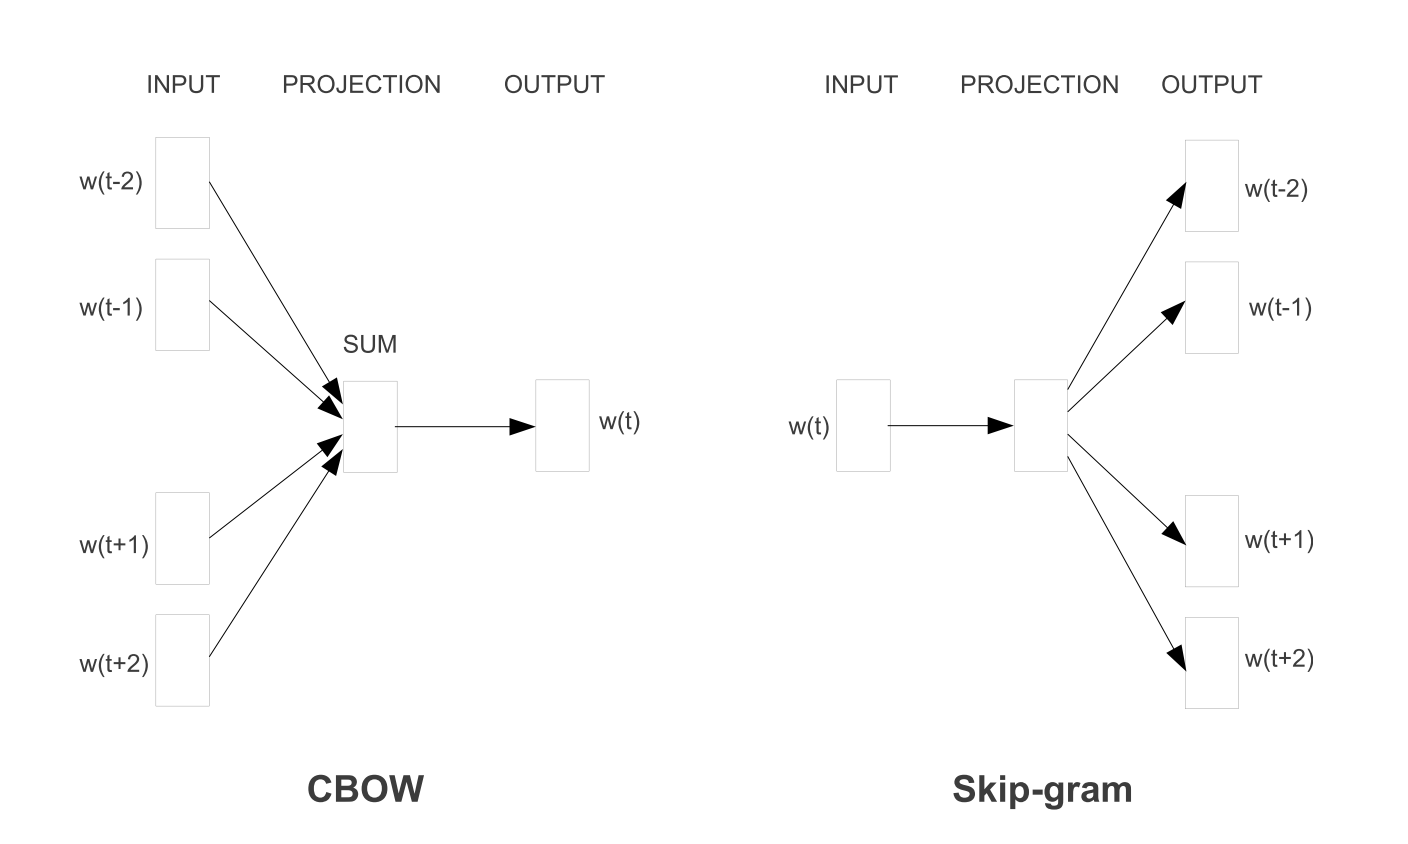
\includegraphics[width=12cm]{kapitel3/cbowskipgr.png}
    \caption[Vergleich zwischen CBOW und Skip-Gram Architektur]{Die CBOW-Architektur sagt das aktuelle Wort basierend auf dem Kontext voraus, während das Skip-Gramm die umgebenden Wörter voraussagt, wenn das aktuelle Wort gegeben ist aus \cite*{Mikolov}).}
    \label{cbowskipgr}
\end{figure}

Der Skip-Gram-Algorithmus ist einer von zwei Algorithmen in einem Softwarepaket namens \textbf{word2vec} \cite*{Mikolov2013}\cite*{Mikolov}. Die Intuition von word2vec ist, dass anstatt zu zählen, wie of jedes Wort $w$ in der Nähe von einem anderen Wort vorkommt, einen Klassifikator für eine binäre Vorhersageaufgabe zu trainieren. Die erlernten Klassifikatorgewichte werden dann als Worteinbettungen genommen \cite*[111]{Jurafskya}. Dabei wird ein Zielwort $t$ mit Kandidaten aus dem Kontext \textit{c} in ein \textit{Tupel} gesetzt. \textit{P(+|t,c)} sagt dann aus, wie wahrscheinlich es ist, dass ein Kontextwort \textit{c} ein echter Kontext ist. Zum Beispiel sei gegeben der Satz \enquote{Wir essen Spaghetti zum Abendessen...}. Wenn der Kontext von $\pm 2$ Wörter betrachtet wird, und \textit{t} das Zielwort \enquote{essen} ist, wird die Klassifikation für das Tupel \textit{(essen,spaghetti)} \enquote{true} und für das Tupel \textit{(essen,auto)} \enquote{false} zurückgeben \cite*[111]{Jurafskya}.

\begin{equation} \label{Formel3_1}
    P(-|t,c) = 1-P(+|t,c)
\end{equation}

Die Ähnlichkeit eines Wortes zu einem anderen Wort, kann mittels Skalarprodukt berechnet werden. Dies ist zunächst nur eine Zahl zwischen $-\infty$ und $+\infty$. Um daraus eine Wahrscheinlichkeit zu berechnen, wird die \textit{sigmoid} Funktion $\sigma(x)$ angewendet. Die Logistikfunktion gibt eine Zahl zwischen 0 und 1 zurück. Um die Wahrscheinlichkeit zu berechnen, muss gewährleistet werden, dass die Summe \textit{c ist das Kontextwort} und \textit{c ist nicht das Kontextwort} eine 1 ergeben \cite*[112]{Jurafskya}.

\begin{equation} \label{Formel3_2}
    P(-|t,c) = 1-P(+|t,c) = \frac{e^{-t\cdot c}}{1+e^{-t\cdot c}}
\end{equation}

Skip-Gramm macht die starke, aber sehr nützliche vereinfachende Annahme, dass alle Kontextwörter unabhängig sind, so dass ihre Wahrscheinlichkeiten multipliziert werden können:

\begin{equation} \label{Formel3_3}
    P(+|t,c_{1:k}) = \prod ^{k}_{i=1}\frac{1}{1+e^{-t\cdot c_{i}}}
\end{equation}

\begin{equation} \label{Formel3_4}
    \log P(+|t,c_{1:k}) =\sum ^{k}_{i=1} \log \frac{1}{1+e^{-t\cdot c_{i}}}.
\end{equation}


Word2vec lernt Einbettungen, indem es mit einem anfänglichen Satz von Einbettungsvektoren beginnt und dann die Einbettung jedes Wortes $w$ iterativ verschiebt, um mehr in der Nähre der Einbettungen von Wörtern zu kömmen die ähneln. Für das Training eines binären Klassifikators werden negative Beispiele nötig. Das Skip-Gram benötigt mehr negative als positive Beispiele für das Training. Das Verhältnis zwischen positiven und negativen Beispielen wird mit einem Parameter $k$ festgelegt. Für jedes der Trainingseinheiten \textit{t, c} werden \textit{k} negative Stichproben erstellt, die jeweils aus dem Ziel \textit{t} und einem \enquote{noise word} besteht. Ein \enquote{noise word} is ein zufälliges Wort aus dem Lexikon, das nicht das Zielwort \enquote{t} sein darf \cite*[113]{Jurafskya}.

Das Ziel des Lernalgorithmus besteht darin, mittels gegebenen positiven und negativen Beispielen diese Einbettungen so anzupassen, dass die Ähnlichkeit der Ziel- und Kontextwortpaare \textit{(t, c)} aus den positiven Beispielen maximiert werden und die Ähnlichkeit der Paare \textit{(t, c)} aus den negativen Beispielen minimiert wird. Formell lässt sich dieses mit folgender Formel ausdrücken:

\begin{gather} \label{Formel3_5}
    L(\theta) = \sum_{(t,c)\in +}\log P(+|t,c)+\sum_{(t,c)\in -} \log P(-|t,c) =  \notag\\
    \log \sigma(c \cdot t)+\sum^{k}_{i=1}\log \sigma(-n_{i} \cdot t) = \notag\\
    \log \frac{1}{1+e^{-c \cdot t}}+\sum^{k}_{i=1}\log\frac{1}{1+e^{n_{1} \cdot t}}.
\end{gather}

Die stochastische Gradientenabstieg kann verwendet werden, um dieses Ziel zu erreichen, indem die Parameter (die Einbettungen für jedes Zielwort $t$ und jedes Kontextwort oder \enquote{noise word} $c$ im Vokabular) iterativ modifiziert werden \cite*[114]{Jurafskya}.


\section{CNN in der Textverarbeitung}
Anstelle von Bildpixeln können die Eingaben für die meisten NLP-Aufgaben Sätze oder Dokumente, als eine Matrix dargestellt werden. Jede Zeile der Matrix entspricht einem Token, normalerweise einem Wort, aber es kann sich auch um ein Zeichen handeln. Das heißt, jede Zeile ist ein Vektor, der ein Wort darstellt. Typischerweise sind diese Vektoren Worteinbettungen (niedrigdimensionale Darstellungen) wie word2vec oder GloVe, aber sie können auch One-Hot-Vektoren sein, die das Wort in ein Vokabular indizieren. Für einen 10-Wort-Satz unter Verwendung einer 100-dimensionalen Einbettung hätten wir eine 10 × 100-Matrix als Eingabe \cite*{Zhang}.

In der Vision \enquote{gleiten} die Filter über lokale \enquote{pathces} eines Bildes, in NLP wird jedoch der Filter über die ganze Zeilen der Matrix (Wörter) gleiten. Daher entspricht die Breite der Filter normalerweise der Breite der Eingabematrix. Die Höhe oder Regionsgröße kann variieren, aber \enquote{Schiebefenster} mit jeweils mehr als 2-5 Wörtern sind typisch. Pixel, die nahe beieinander liegen, sind wahrscheinlich semantisch verwandt (Teil desselben Objekts), aber das Gleiche gilt nicht immer für Wörter. In vielen Sprachen können Teile von Phrasen durch mehrere andere Wörter getrennt werden. Der kompositorische Aspekt ist ebenfalls nicht offensichtlich. Es ist klar, dass Wörter in gewisser Weise zusammengesetzt sind, wie ein Adjektiv, das ein Substantiv modifiziert, aber wie genau dies funktioniert, was Darstellungen auf höherer Ebene tatsächlich \enquote{bedeuten}, ist nicht so offensichtlich wie im Fall von Computer Vision. Angesichts all dessen scheinen CNNs nicht gut für NLP-Aufgaben geeignet zu sein. Wiederkehrende neuronale Netze (RNNs) sind intuitiver. Sie ähneln der Art und Weise, wie wir Sprache verarbeiten (oder zumindest wie wir denken, dass wir Sprache verarbeiten). Lesen nacheinander von links nach rechts. Glücklicherweise bedeutet dies nicht, dass CNNs nicht funktionieren. Alle Modelle sind falsch, aber einige sind nützlich. Es stellt sich heraus, dass CNNs, die auf NLP-Probleme angewendet werden, recht gut funktionieren. Ein großes Argument für CNNs ist, dass sie schnell sind. Faltungen sind ein zentraler Bestandteil der Computergrafik und werden auf Hardwareebene auf GPUs implementiert. Mit einem großen Wortschatz kann das Berechnen schnell \enquote{teuer} werden. Faltungsfilter lernen automatisch gute Darstellungen, ohne das gesamte Vokabular darstellen zu müssen \cite*{widlml}.

\begin{figure}[H]
    \centering
    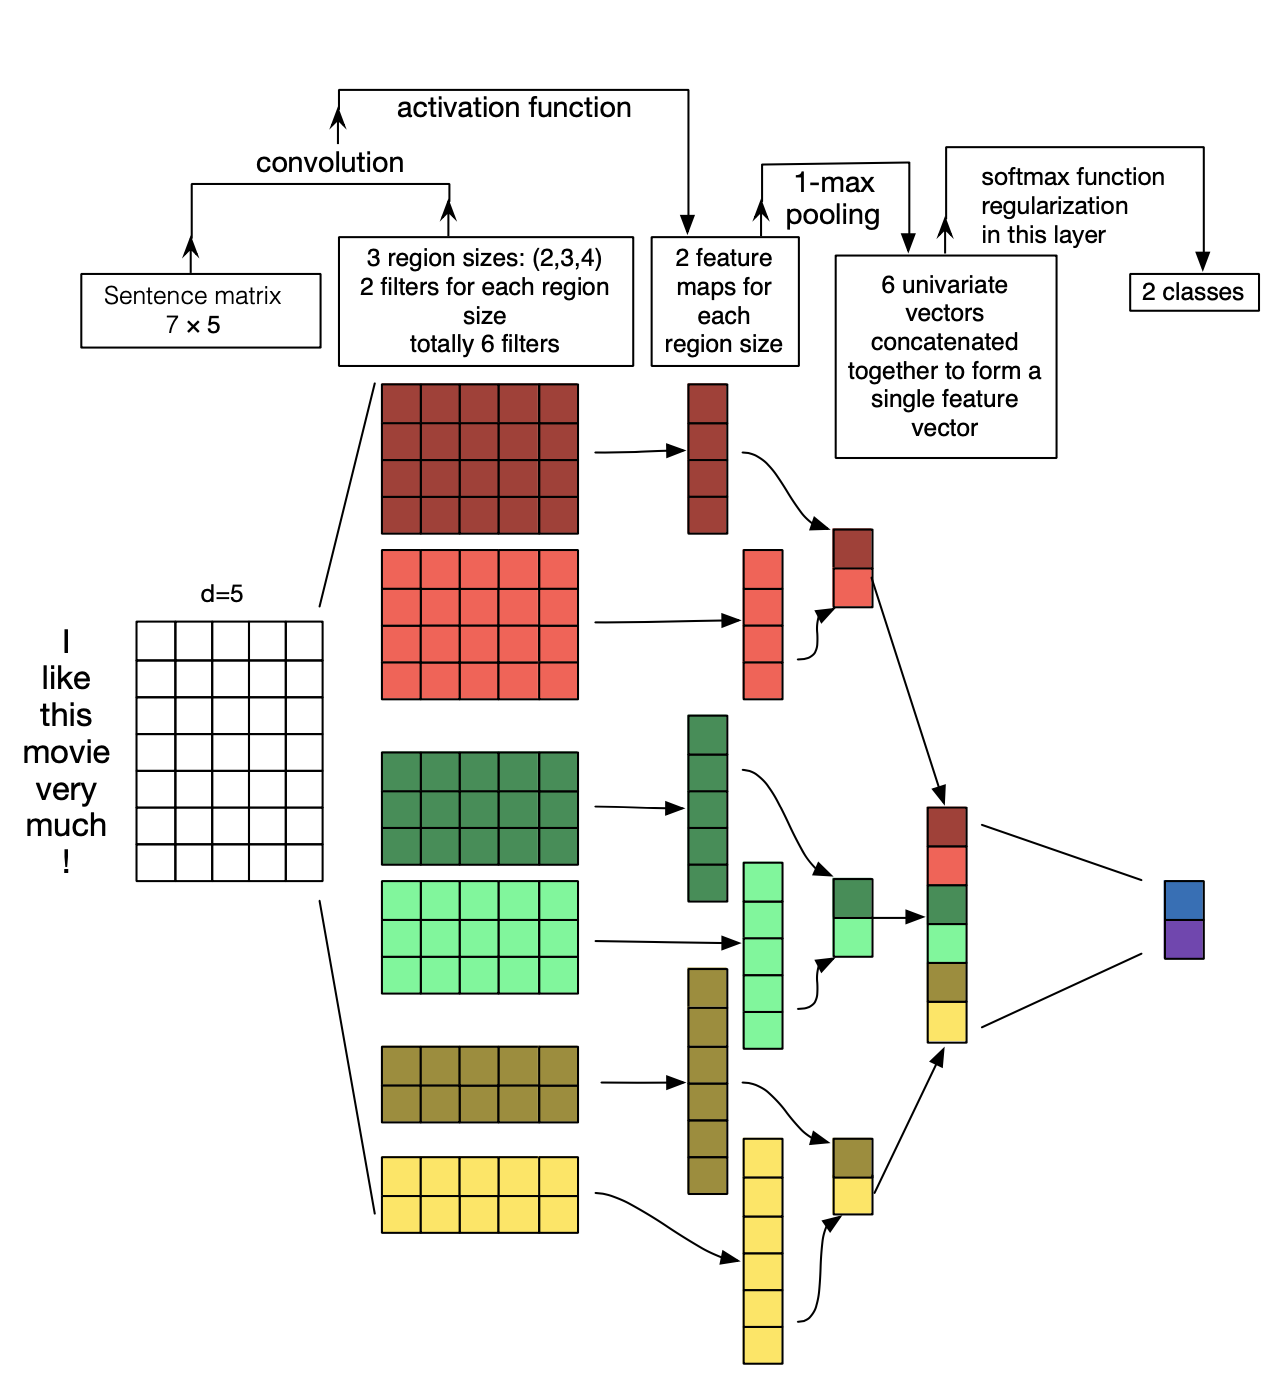
\includegraphics[width=10cm]{kapitel2/cnnnlp.png}
    \caption[CNN in der Textverarbeitung]{Illustration einer CNN-Architektur zur Satzklassifizierung. Es sind drei Filterbereichsgrößen vorhanden: 2, 3 und 4. Filter führen Faltungen in der Satzmatrix durch und generieren Feature-Maps (mit variabler Länge). Über jede Karte wird ein 1-Max-Pooling durchgeführt, d. H. die größte Anzahl von jeder Merkmalskarte wird aufgezeichnet. Somit wird aus allen sechs Karten ein univariater Merkmalsvektor erzeugt, und diese sechs Merkmale werden verkettet, um einen Merkmalsvektor für die vorletzte Schicht zu bilden. Die letzte Softmax-Schicht empfängt dann diesen Merkmalsvektor als Eingabe und verwendet ihn zur Klassifizierung des Satzes an. Hier wird eineeine binäre Klassifikation angewendet und es gibt daher zwei mögliche Ausgangszustände dar \cite*{Zhang}.}
    \label{Kap2:Pooling}
\end{figure}

% \subsubsection{Glove}
% Eine andere Methode zum Einbetten von Wörtern ist Glove (\enquote{Global Vectors}). Es basiert auf Matrixfaktorisierungstechniken für die Wortkontextmatrix. Zunächst wird eine große Matrix von Informationen zum gleichzeitigen Auftreten von Wörter und Kontext erstellt, d. H. für jedes \enquote{Wort} (die Zeilen) wird gezählt, wie häufig dieses Wort in einem \enquote{Kontext} (den Spalten) in einem großen Korpus angezeigt wird. Dann wird diese Matrix in eine niederdimensionale Matrix Wort und Merkmale zerlegt, in der jede Zeile nun eine Vektordarstellung für jedes Wort speichert. Dies geschieht im Allgemeinen durch Minimierung eines \enquote{Rekonstruktionsverlusts}. Dieser Verlust versucht, die niederdimensionalen Darstellungen zu finden, die den größten Teil der Varianz in den hochdimensionalen Daten erklären können.




% \chapter{Grobe Zeit- und Ressourcenplanung}
% % \label{Kap3}
% Grobe Zeitplanung und die Anteile der Kapitel and er Arbeit:
% \begin{itemize}
%     \item \textbf{November 2020 bis Oktober 2020:} Kapitel 2, 3 (ca. 25\%)
%     \item \textbf{Dezember 2020} Kapitel 4-5 (ca. 25\%)
%     \item \textbf{Januar 2021:} Kapitel 6 (ca. 20\%)
%     \item \textbf{Februar 2021:} Kapitel 7 (ca. 20\%)
%     \item \textbf{März 2021:} Kapitel 1, 8 (ca. 10\%)
% \end{itemize}
% \section{Bilder}

% Natürlich können auch Grafiken und Bilder eingebunden werden, siehe z.\,B. Abbildung~\ref{Kap2:NasaRover}.

% \begin{figure}[ht]
%     \centering
%     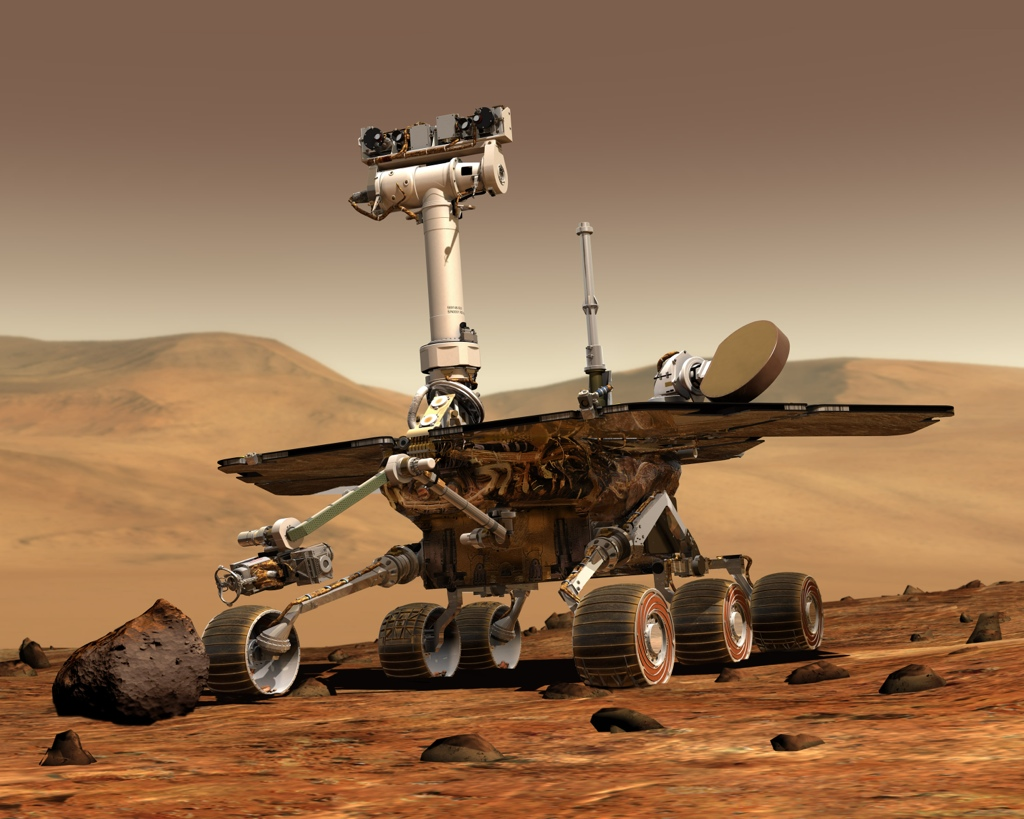
\includegraphics[width=6cm]{kapitel3/nasa_rover}
%     \caption{Ein Nasa Rover}
%     \label{Kap2:NasaRover}
% \end{figure}

% Man kann sich auch selbst ein Makro für das Einfügen von Bildern schreiben:

% \bild{kapitel3/modell_point_to_point}{6cm}{Point to Point}

% \begin{sidewaysfigure}
%     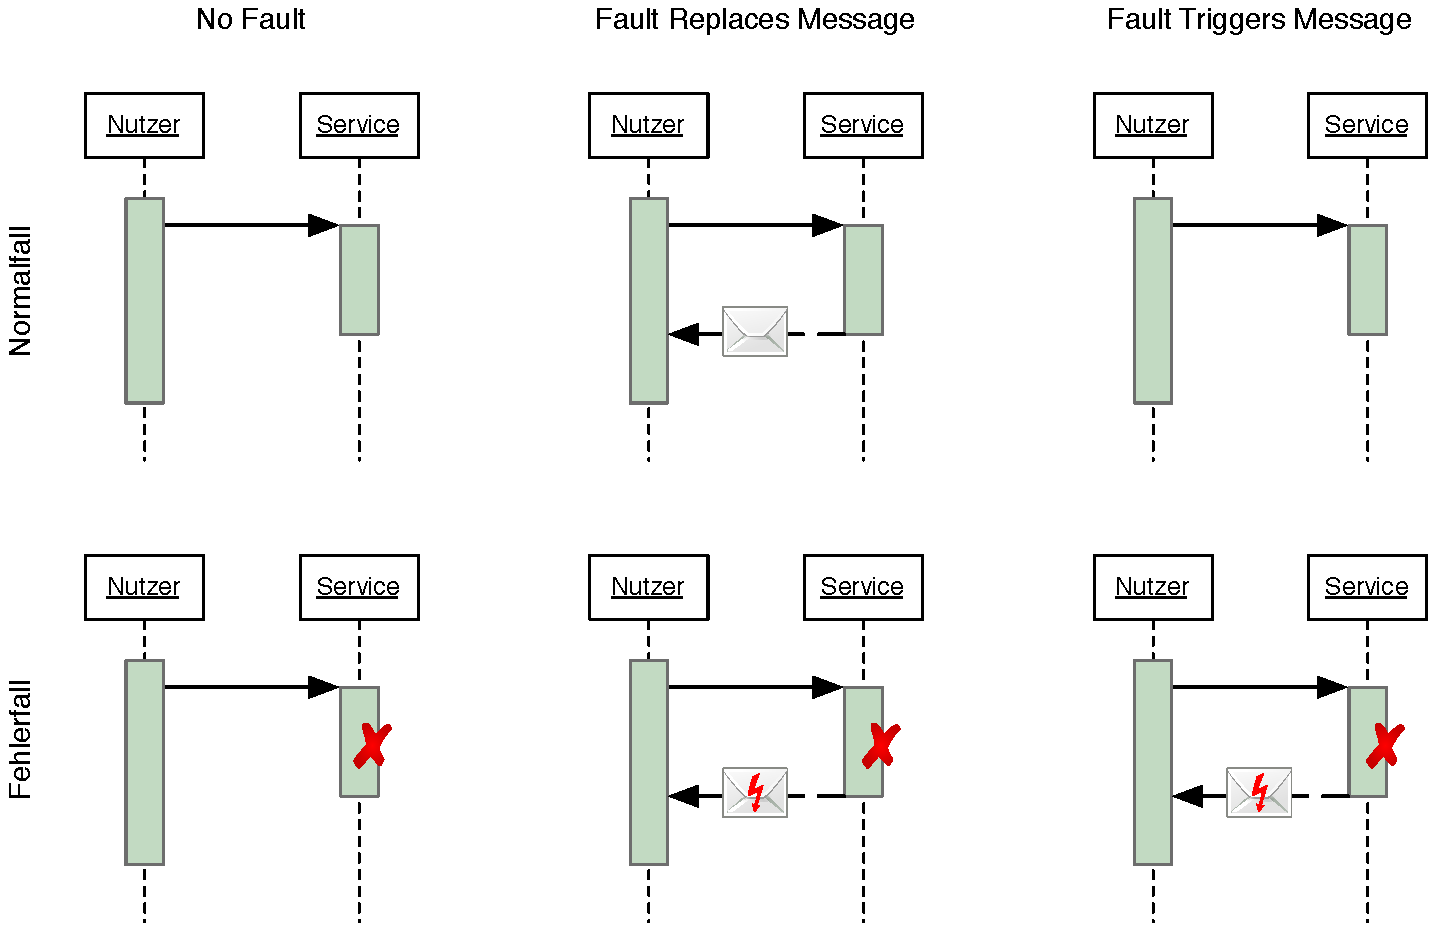
\includegraphics[width=22cm]{kapitel3/ws-wsdl20-fehler}
%     \caption{Sehr große Grafiken kann man drehen, damit sie auf die Seite passen}
%     \label{Kap2:wsdl-fehler}
% \end{sidewaysfigure}

% \clearpage % Alle Bilder, die bisher kamen ausgeben


% \section{Formelsatz}

% Eine Formel gefällig? Mitten im Text $a_2 = \sqrt{x^3}$ oder als eigener Absatz (siehe Formel~\ref{Formel}):

% \begin{equation}
%     \begin{bmatrix}
%         1 & 4 & 2  \\
%         4 & 0 & -3
%     \end{bmatrix}
%     \cdot
%     \begin{bmatrix}
%         1  & 1 & 0 \\
%         -2 & 3 & 5 \\
%         0  & 1 & 4
%     \end{bmatrix}
%     {=}
%     \begin{bmatrix}
%         -7 & 15 & 28  \\
%         4  & 1  & -12
%     \end{bmatrix}
%     \label{Formel}
% \end{equation}


% \section{Sourcecode}

% Man kann mit Latex auch ganz toll Sourcecode in den Text aufnehmen.

% \subsection{Aus einer Datei}

% \lstinputlisting[firstline=2,language=Java,caption={Crypter-Interface},label=lst:CrypterInterface]{\srcloc/Crypter.java}


% \subsection{Inline}

% \begin{lstlisting}[language=Java,caption=Methode checkKey()]
%     /**
%      * Testet den Schlüssel auf Korrektheit: Er muss mindestens die Länge 1
%      * haben und darf nur Zeichen von A-Z enthalten.
%      *
%      * @param key zu testender Schlüssel
%      * @throws CrypterException wenn der Schlüssel nicht OK ist.
%      */
%     protected void checkKey(Key key) throws CrypterException {

%         // Passt die Länge?
%         if (key.getKey().length == 0) {
%             throw new CrypterException("Der Schlüssel muss mindestens " +
%                     "ein Zeichen lang sein");
%         }

%         checkCharacters(key.getKey(), ALPHABET);
%     }
% \end{lstlisting}


% \section{Anforderungen}

% Anforderungen im Format des Volere"=Templates (Snowcards) \autocite{Volere} können per Makro eingefügt werden. Das Label wird automatisch mit der Nummer erstellt, d.\,h. Sie können auf die Tabelle mit dieser referenzieren (siehe \autoref{F52}).

% \snowcard % Snowcard einbinden (Anpassungen in titelblatt.tex)
% {F52} % Nummer des Requirements
% {F} % Art
% {Hoch} % Priorität
% {User Authentifizierung} % Titel
% {Interview mit Abteilungsleiter} % Herkunft (Optional)
% {F12} % Konflikte (Optional)
% {Der Benutzer ist in der Lage sich über seinen
%     Benutzernamen und sein Passwort am System anzumelden} % Beschreibung
% {Ein Benutzer kann sich mit seinem firmenweiten Benutzernamen und
%     Passwort über die Anmeldemaske anmelden und hat Zugriff auf die
%     Funktionen des Systems} % Fit-Kriterium (Optional)
% {Benutzerhandbuch des Altsystems} % Material (Optional)

% Ebenso können Sie nicht"=funktionale Anforderungen mit Hilfe von Quality Attribute Scenarios (vgl. \autoref{NF11}) darstellen. Zu Details siehe \autocite{Barbacci2003}.

% \qas % Quality-Attribute Scenario einbinden (Anpassungen in titelblatt.tex)
% {NF11} % Nummer des Requirements
% {Hoch} % Priotität
% {Performance des Jahresabschlusses} % Titel
% {Endbenutzer} % Quelle
% {Startet einen Jahresabschluss} % Stimulus
% {Buchhaltungssystem} % Artefakt
% {Das System befindet sich im normalen Betriebszustand} % Umgebung
% {Jahresabschluss ist durchgeführt und kann als PDF abgerufen werden} % Antwort
% {10 Minuten} % Antwort-Maß

% Die Abgrenzung von funktionalen und nicht-funktionalen Anforderungen ist nicht immer einfach und bereitet manchen Studierenden Probleme. Als Hilfestellung kann die von der ISO25010 \autocite{ISO25010} zur Verfügung gestellte Liste dienen, siehe \autoref{kapitel3/iso25010}.

% \bild{kapitel3/iso25010}{14cm}{Qualitätsmodell für Software-Produkte nach ISO25010}

% \citeauthor{Bass2003} listen in \autocite{Bass2003} eine ähnliche Liste von Kategorien für nicht-funktionalen Anforderungen auf, die ebenfalls als Richtschnur dienen kann. Diese sind:

% \begin{itemize}
%     \item \textit{Verfügbarkeit} \textit{(availability)} -- umfasst Zuverlässigkeit (reliability), Robustheit (robustness), Fehlertoleranz (fault tolerance) und Skalierbarkeit (scalability)
%     \item \textit{Anpassbarkeit} \textit{(modifiability)}, umfasst Wartbarkeit (maintainability), Verständlichkeit (understandability) und Portabilität (portability).
%     \item \textit{Performanz} \textit{(performance)}
%     \item \textit{Sicherheit} \textit{(security)}
%     \item \textit{Testbarkeit} \textit{(testability)}
%     \item \textit{Bedienbarkeit} \textit{(usability)}
% \end{itemize}
 % Externe Datei einbinden

\chapter{Verwandte Arbeiten}% \chapter{Checkliste}


\section{Einleitung}
Clickbaits besitzen semantische und syntaktische Nuancen, auf die besonders vorgegangen werden muss. Dies geschieht in Form von analyse und vorverarbeitung der Titel. In diesem Abschnitt werden Ansätze aus der Literatur verglichen, die diese semantischen und syntaktischen Besonderheiten bearbeiten. In diesem Kapitel werden Ansätzte aus der Literatur vorgestellt, die die Aufgabe Clickbait Klassifizierung und die damit entstehenden Unteraufgaben wie das Sammeln von Daten, Einbetten der Wörter und schließlich entwickeln der Deep Learning Modelle haben.


\section{Analyse der Literatur}
Mit der Arbeit aus \cite*{Chakrabortya} wurde eine Browser-Erweiterung erstellt, welches Clickbaits erkennen soll. Es wurden umfangreiche Daten sowohl für Clickbaits als auch für Nicht-Clickbait-Kategorien gesammelt. Für die Nicht-Clickbaits-Kategorien wurden 18.513 Wikinews Artikeln gesammelt. Der Vorteil dieser Artikel ist, dass diese von einer Community erstellt werden und jeder Nachrichtenartikel vor der Veröffentlichung von der Community geprüft werden. Es gibt Stilrichtlinien, die eingehalten werden müssen. Um Clickbaits zu finden, haben die Autoren manuell aus Seiten wie \enquote{Buzzfeed} oder \enquote{Upworthy} ca. 8000 Titel gecrawlt. Um falsche Negative zu vermeiden (d. h. die Artikel in diesen Bereichen, bei denen es sich nicht um Clickbaits handelt), wurden sechs Freiwillige rekrutiert um die Überschriften zu labeln. Schließlich wurden 7500 Titel zu jeder der beiden Kategorien zugefügt.

% \section{Analyse Textdaten}


Laut \cite*{Chakrabortya} sind die herkömmlichen Nicht-Clickbait Schlagzeilen kürzer als Clickbait Schlagzeilen. Traditionelle Schlagzeilen enthalten in der Regel meistens Wörter, die sich auf bestimmte Personen und Orte beziehen, während die Funktionswörter den Lesern zur Interpretation aus dem Kontext überlassen bleiben. Es wird hier als Beispiel gegeben \enquote{Visa-Deal oder kein Migranten-Deal, Türkei warnt EU}. Hier sind die meisten Wörter Inhaltswörter, die die wichtigsten Erkenntnisse aus der Geschichte zusammenfassen, und es gibt nur sehr wenige Verbindungsfunktionswörter zwischen den Inhaltswörtern. Auf der anderen Seite sind Clickbait Schlagzeilen länger. Die Sätze, enthalten sowohl Inhalts- als auch Funktionswörter. Ein Beispiel für solche Schlagzeilen ist \enquote{Ein 22-Jähriger, dessen Ehemann und Baby von einem betrunkenen Fahrer getötet wurden, hat ein Facebook-Plädoyer veröffentlicht}. Obwohl die Anzahl der Wörter in Clickbait-Schlagzeilen höher ist, ist die durchschnittliche Wortlänge kürzer. Es werden häufig Wörter verwendet wie \enquote{Sie werden}, \enquote{Sie sind}. Im Durchschnitt haben die Wörter bei den Clickbaits längere Abhängigkeiten als Nicht-Clickbaits. Der Hauptgrund ist die Existenz komplexerer Phrasensätze im Vergleich zu Schlagzeilen ohne Clickbait. Es ist außerdem zu sehen, dass in Clickbait-Schlagzeilen Stoppwörter häufiger verwendet werden. Clickbait Überschriften verwenden häufig Determinantien wie \enquote{ihre}, \enquote{meine}, die auf bestimmte Personen oder Dinge im Artikel verweisen. Die Verwendung Wörter dient in erster Linie dazu, den Benutzer neugierig auf das Objekt zu machen, auf das verwiesen wird, und ihn zu überzeugen, den Artikel weiter zu verfolgen. Um Daten zu erfassen, können auch Soziale Medien wie Twitter herangezogen werden, wie im Beispiel von \cite*{Potthast}.


% \section{Feature Selection}
Um lexikalischer und semantische und orthografische und morphologische Merkmale zu erfassen, benutzen die Autoren aus \cite*{Anand2019} Worteinbettungen und Zeicheneinbettungen, anstatt übermäßig Feature Selection auszuüben. Um Informationen außerhalb einzelner oder fester Wortfenster zu erfassen, untersuchten die Autoren dabei verschiedene RNN-Architekturen (Recurrent Neural Network) wie LSTM (Long Short Term Memory), GRU (Gated Recurrent Units) und Standard-RNNs. Dieses sind Wiederkehrende neuronale Netzwerkmodelle, die für sequentielle Daten wie Sprache und Text gut modelliert werden können.


Die Arbeit von \cite*{Agrawal2017} schlägt ein Modell vor, welches CNNs benutzt. CNNs werden für verschiedene Deep-Learning-Aufgaben verwendet. Es wurde nur eine Faltungsschicht in das CNN-Modell eingebaut. Die erste Schicht wird für das Einbetten der Wörter in Vektoren verwendet. Dabei wurden 2 verschiedene Worteinbettungen in Bezug genommen. Ein vortrainiertes und eines welches von Grund auf lernen musste und sich während des Trainings weiterentwickelt. In der nächsten Schicht werden Filter in verschiedenen Größen verwendet um Faltungen über Wortvektoren zu erzeugen.

Die Autoren der Arbeit aus \cite*{Pujahari} Clustern zunächst die aus den Schlagzeilen erstellten Vektoren mit der sogenannten t-SNE Methode nach \cite{VanDerMaaten2008}. Dieser Algorithmus \enquote{rekategorisiert} die Schlagzeilen in mehrere Gruppen und reduziert die vielen Dimensionen von Clickbaits im Datensatz. Die Autoren beginnen erst im nächsten Schritt mit dem Training. Dabei entstehen 11 Kategorien von Clickbaits (Mehrdeutig, Übertreibung oder Neckerei).


\begin{figure}[H]
    \centering
    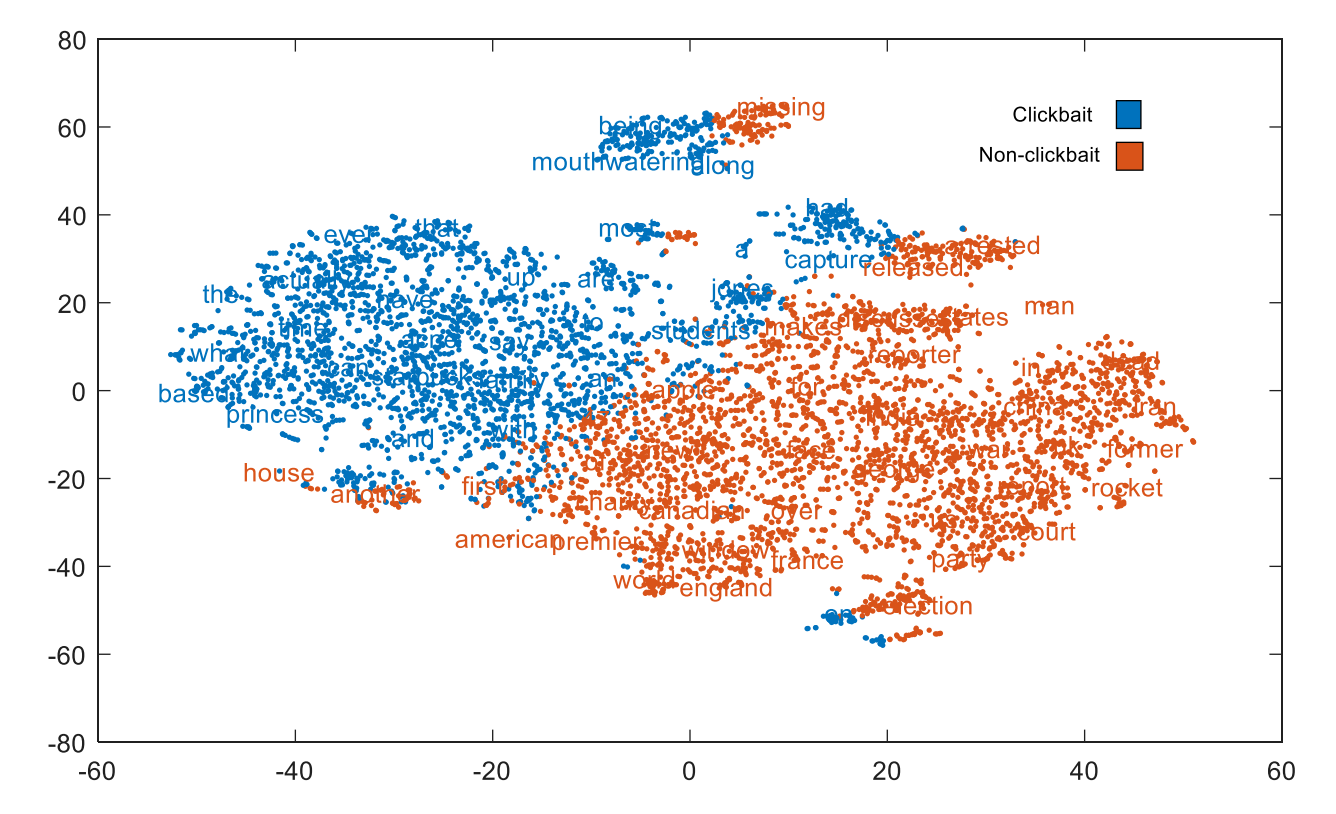
\includegraphics[width=12cm]{kapitel4/tsne.png}
    \caption[Clustering von Überschriften mit t-SNE]{Die Autoren verwenden das t-SNE Algorithmus nach \cite{VanDerMaaten2008} um die Dimensionen zu Reduzieren und es entstehen mehrere Unterkategorien von Clickbaits. Entnommen aus \cite*{Pujahari}.}
    \label{TSNE}
\end{figure}

\section{Schluss}
In diesem Kapitel wurden einige Arbeiten aus der Literatur vorgestellt, jedoch nicht alle. Es gibt außerdem noch weitere Arbeiten wie \cite*{chawda2019novel}\cite*{Zannettou2018}\cite*{Kumar}\cite*{Thomas}\cite*{Liao}\cite*{Glenski} und \cite*{Biyani2016} die unter diese Literaturstudie fallen könnten. Alle diese Arbeiten in Ihrer ganzen Fülle zu beschreiben würde den Rahmen dieser Arbeit sprengen, sodass nur ein Einblick über mögliche Aufgaben, wie das Sammeln von Daten und das Bauen eines Deep Learning Ansatzes sowie die Besonderheiten die Clickbaits Schlagzeilen haben, verschafft wurde.


% \section{Anwendung von Deep Learning Modellen}


% \label{Kap4}

% Die folgende Checkliste kann dazu dienen, die Arbeit auf die wichtigsten Bewertungskriterien zu prüfen. Jeder Dozent hat andere Kriterien, die unten aufgeführten dürften aber für die meisten Dozenten gültig sein.

% \section{Form und Sprache}

% \begin{checklist}
%   \footnotesize
%   \item \textbf{Aufbau}: Die Arbeit ist nach wissenschaftlichen Prinzipien aufgebaut (wesentliche Teile vorhanden, Nummerierung/Verweise korrekt, Verzeichnisse vorhanden).
%     \begin{checklist}
%         \item \textit{Wesentliche Teile}: Die folgenden Elemente der Arbeit sind vorhanden: Titelblatt, Abstract/Zusammenfassung, Einleitung, Hauptteil, Fazit/Ausblick.
%         \item \textit{Nummerierung/Verweise}: Das Nummerierungsschema wird konsistent über die gesamte Arbeit durchgehalten, die Verweise auf die verschiedenen Elemente (Abbildungen, Tabellen etc.) sind korrekt.
%         \item \textit{Verzeichnisse}: Die Arbeit enthält alle relevanten Verzeichnisse: Inhaltsverzeichnis, Literaturverzeichnis, Abbildungsverzeichnis, Tabellenverzeichnis, eventuell Glossar.
%     \end{checklist}
%   \item \textbf{Sprache}: Die verwendete Sprache entspricht wissenschaftlichen Ansprüchen.
%     \begin{checklist}
%         \item \textit{Begriffe und Definitionen}: Begriffe werden einheitlich und konsistent verwendet. Neue Begriffe werden definiert und mit Literatur hinterlegt.
%         \item \textit{Abkürzungen}: Alle Abkürzungen werden eingeführt und erläutert. Abkürzungen werden bei der ersten Verwendung ausgeschrieben und in einem Abkürzungsverzeichnis geführt. Es werden keine unüblichen oder selbst erfunden Abkürzungen verwendet. Ein Glossar kann verwendet werden, um Begriffe noch einmal kompakt darzustellen.
%         \item \textit{Rechtschreibung}: Die Arbeit ist frei von Rechtschreibungs-, Zeichensetzungs- und Grammatikfehlern.
%     \end{checklist}
%   \item \textbf{Formatierung, Typographie}: Die Formatierung der Arbeit ist korrekt und aus typographischer Sicht einwandfrei. \textit{Wenn Sie dieses Template korrekt verwenden, sollte dieser Punkt automatisch durch die Verwendung von \LaTeX \ erledigt sein.}
%     \begin{checklist}
%         \item \textit{Korrekte Typographie}: Schriftarten werden korrekt verwendet (nicht mehr als 2 Fonts), der Zeilenabstand ist passend, die Ränder sind ausreichend, der Satz ist korrekt.
%         \item \textit{Satz von Abbildungen, Tabellen etc.}: Abbildungen sind in der richtigen Auflösung dargestellt, die Tabellen sind korrekt gesetzt, mathematische Formeln und Symbole sind sauber dargestellt.
%     \end{checklist}
%   \item \textbf{Abbildungen}: Abbildungen werden in ausreichendem Umfang zur Förderung des Verständnisses eingesetzt. Sie werden korrekt im Text referenziert und sind, wo immer möglich, in einer Standardnotation erstellt.
%     \begin{checklist}
%         \item \textit{Ausreichende Verwendung}: Komplizierte Sachverhalte werden durch Abbildungen verdeutlicht. Es werden genug Abbildungen eingesetzt, um die wichtigsten Sachverhalte zu erklären.
%         \item \textit{Verständnisförderung}: Abbildungen dienen nicht als Schmuck, sondern um komplizierte Sachverhalte zu verdeutlichen.
%         \item \textit{Einbindung in den Text}: Der Text muss auch ohne Abbildungen verständlich sein, die Abbildungen helfen Sachverhalte aus dem Text besser darzustellen. Der Text referenziert die Abbildung korrekt.
%         \item \textit{Standardnotation, Legende}: Die Abbildungen verwenden Standard"=Notationen wie UML, FMC etc. Wo keine Standardnotation eingesetzt wird, ist eine Legende vorhanden, um die Bildelemente zu erläutern.
%     \end{checklist}
%   \item \textbf{Zitate}: Quellen werden konsistent nach einer gängigen Zitierweise zitiert und sind vollständig im Literaturverzeichnis angegeben.
%     \begin{checklist}
%         \item \textit{Zitierweise}: Die Zitierweise in der gesamten Arbeit folgt einem einheitlichen Schema, z.B. IEEE, DIN, Chicago.
%         \item \textit{Vollständigkeit}: Alle Zitate sind als solche kenntlich gemacht und die Quelle wird vollständig angegeben, und Plagiate werden vermieden.
%     \end{checklist}
%   \item \textbf{Schreibstil}: Lebendiger, wissenschaftlicher und verständlicher Schreibstil.
%     \begin{checklist}
%         \item \textit{Wissenschaftlichkeit}: Der Text ist im Präsenz geschrieben, es wird die dritte Person verwendet, Fachausdrücke werden korrekt verwendet, Fremdwörter und Amerikanismen werden richtig eingesetzt.
%         \item \textit{Verständlichkeit}: Abschweifungen und Wiederholungen werden vermieden, statt dessen werden präzise und übersichtliche Sätze verwendet.
%         \item \textit{Lebendigkeit}: Der Text der Arbeit zeichnet sich durch eine gute Wortwahl, Sprachbilder, einen angemessenen Satzbau und eine hohe Variabilität aus.
%     \end{checklist}
% \end{checklist}

% \section{Inhalt}

% \begin{checklist}
%   \footnotesize
%   \item \textbf{Gliederung}: Die Gliederung ist vollständig, konsistent und sachlogisch mit angemessener Struktur und Tiefe.
%     \begin{checklist}
%         \item \textit{Konsistenz und Vollständigkeit}: Auf einer Ebene stehen keine Punkte alleine, die Gliederungspunkte orientieren sich an der Argumentationskette.
%         \item \textit{Angemessene Tiefe}: Die Größe der einzelnen Unterpunkte ist vom Umfang her ähnlich. Es gibt keine Gliederungspunkte, die nur aus ein bis zwei Sätzen bestehen.
%     \end{checklist}
%   \item \textbf{Grundlagen}: Es werden alle relevanten Grundlagen gelegt. Der State"=of"=the"=art und der State"=of"=practice werden dargelegt.
%     \begin{checklist}
%         \item \textit{Umfang}: 1/3 des Hauptteils ist ein gutes Maß für eine ausreichende Darstellung der Grundlagen.
%         \item \textit{Begriffe und Methoden}: Begriffe und Methoden sind definiert, und Literatur zu den Definitionen ist angegeben.
%         \item \textit{State-of-the-art}: Der Stand des verfügbaren Wissens wird dargestellt, analysiert und kritisch beurteilt (state-of-the-art). Bei theoretischen Arbeiten kann ein eigenes Kapitel \enquote{verwandte Arbeiten} nötig sein, um den state"=of"=the"=art darzustellen.
%         \item \textit{State-of-practice}: Bei praktischen Arbeiten, die in der Industrie geschrieben werden, kann es nötig sein, auch das Vorgehen im Unternehmen zu erläutern.
%     \end{checklist}
%   \item \textbf{Methodik/Lösung}: Die gewählte Methodik bzw. Lösung ist für das Problem adäquat.
%     \begin{checklist}
%         \item \textit{Anforderungen an die Lösung}: Die von der Lösung zu erfüllenden Anforderungen werden dargestellt. Wo nötig wird dies auf Grundlage eines sauberen Requirements"=Engineerings durchgeführt.
%         \item \textit{Erläuterung des Lösungsansatzes}: Der gewählte Lösungsansatz wird ausführlich erläutert und verständlich dargestellt.
%         \item \textit{Eignung zur Lösung der Aufgabe}: Die gewählte Lösung ist geeignet, um das beschriebene Problem zu lösen.
%         \item \textit{Hypothesen}: Es sind ggf. Hypothesen gebildet worden; diese sind erläutert, und es sind Kriterien identifiziert worden, mit deren Hilfe man die Hypothesen falsifizieren kann.
%         \item \textit{Alternativen}: Es werden Alternativen zur vorgeschlagenen Lösung diskutiert. Die eigene Lösung wird nicht als einzige mögliche dargestellt, sondern es werden auch andere mögliche Lösungen vorgestellt und bewertet.
%         \item \textit{Begründung}: Alternativen und Kriterien für die Auswahl dieser Lösung werden dargestellt.
%         \item \textit{Vorteile der Lösung}: Es wird dargestellt, wieso die entwickelt Lösung vorteilhafter ist als die bisherigen Ansätze. Diese Darstellung erfolgt auf Basis des Lösungsansatzes. Eine konkrete Validierung der Implementierung erfolgt ggf. in späteren Kapiteln.
%     \end{checklist}
%   \item \textbf{Logik der Argumentationskette}: Die Argumentation ist logisch und nachvollziehbar. Sie ist frei von logischen Fehlschlüssen.
%   \item \textbf{Implementierung}: Wenn eine Implementierung der Lösung erfolgt, so wird die Implementierung beschrieben. Die Darstellung der Implementierung kann knapp ausfallen. Wichtig ist der Lösungsansatz, nicht die konkrete Umsetzung.
%   \item \textbf{Validierung}: Die vorgeschlagene Lösung wird ggf. empirisch verprobt.
%     \begin{checklist}
%         \item \textit{Vorgehensweise}: Die Vorgehensweise zur Validierung der Lösung / Hypothesen ist beschrieben und geeignet, relevante Aspekte der Lösung zu überprüfen.
%         \item \textit{Empirische Analyse}: Die Erfassungsmethode wird dargestellt und die Daten werden nach den Grundsätzen ordnungsgemäßer Laborpraxis gesammelt und statistisch korrekt ausgewertet.
%         \item \textit{Verprobung}: Die Lösung wird an einem praktischen Beispiel verprobt, und es werden wissenschaftlich korrekte Schlüsse aus der Anwendung gezogen.
%         \item \textit{Zielerreichung}: Funktioniert die gewählte Lösung nach der Implementierung? Wie weit wurde das Ziel erreicht? Falls nicht, gibt es nachvollziehbare Gründe dafür und wurden diese dargestellt?
%     \end{checklist}
%   \item \textbf{Diskussion}: Die Lösung und ihre Validierung wird kritisch und im Kontext möglicher Alternativen diskutiert und bewertet.
%     \begin{checklist}
%         \item \textit{Kritische Reflektion}: Grenzen und Schwächen der eigenen Ergebnisse werden beleuchtet.
%         \item \textit{Ableitung von Konsequenzen}: Die Konsequenzen aus den Ergebnissen für die Wissenschaft und Praxis sind beschrieben.
%     \end{checklist}
%   \item \textbf{Quellenarbeit}: Es werden hochwertige Quellen in ausreichendem Umfang genutzt und kritisch hinterfragt. Eventuell vorhandene Quellen aus dem Unternehmen werden ebenfalls berücksichtigt.
%     \begin{checklist}
%         \item \textit{Umfang}: Der Umfang an Quellen richtet sich stark nach Thema und Art der Arbeit. Bei einer Bachelorarbeit sind mindestens 20 Primärquellen und entsprechend viele Sekundärquellen üblich, bei einer Masterarbeit deutlich mehr.
%         \item \textit{Wissenschaftliche Qualität}: Nicht zitierfähig sind Internet"=Quellen, Wikipedia"=Einträge sowie andere Bachelor- oder Masterarbeiten (sofern nicht veröffentlicht). Das ausschließliche Zitieren von Lehrbüchern ist problematisch. Aktuelle wissenschaftliche Artikel und Werke sollten in den Quellen auftauchen.
%         \item \textit{Quellen \enquote{aus der Praxis}}: Wenn es im Unternehmen spezielle Quellen und Informationen gibt, so werden diese berücksichtigt, z. B. firmen- oder branchenspezifischer Informationen.
%         \item \textit{Kritische Würdigung}: Quellen und Zitate werden kritisch hinterfragt und nicht einfach unreflektiert übernommen. Es gibt eine kritische Distanz bei der Quellenauswahl und Quellenauswertung.
%     \end{checklist}
%   \item \textbf{Fazit}: Es wird eine Zusammenfassung der Arbeit sowie Ausblick auf weitere mögliche Arbeiten im Themenfeld gegeben, etwa die Lösung ausstehender Probleme oder die Erfüllung zusätzlicher Anforderungen.
%   \item \textbf{Umfang der Arbeit}: Richtgrößen: Bachelorarbeiten: 50--80 Seiten, Masterarbeiten: 60--100 Seiten, jeweils ohne Verzeichnisse und Anhang.
% \end{checklist}

% \section{Vor der Abgabe}

% \begin{checklist}
%   \footnotesize
%   \item \textit{Korrektur}: Haben Sie einen Dritten die Arbeit lesen lassen und alle gefundenen Rechtschreib- und Zeichensetzungsfehler behoben?
%   \item \textit{Literaturverzeichnis}: Sind im Literaturverzeichnis irrelevante Informationen entfernt? Beispielsweise bei Büchern unnötige Informationen über die Herkunft bei Google-Books oder bei Papern doppelte Angaben der DOI?
%   \item \textit{Doppel- oder einseitiger Druck}: Entspricht die Einstellung des Templates dem Druck, d.\,h. ist das Template für doppelseitigen Druck eingestellt, wenn doppelseitig gedruckt werden soll und umgekehrt?
%   \item \textit{Umschläge}: Sind die Umschläge vorhanden, um die Arbeit später zu binden? Die Umschläge können in der Hausdruckerei der Hochschule erworben werden.
%   \item \textit{Copyshop}: Wissen Sie, wo Sie die Arbeit drucken werden? Die Hausdruckerei kann Ihre Arbeit nicht drucken.
%   \item \textit{Exemplare}: Haben Sie geklärt, ob der Zweitkorrektor auch ein gedrucktes Exemplar möchte?
% \end{checklist}
 % Externe Datei einbinden
\chapter{Implementierung}
\section{Konzeption und Methodik}


Das Konzept dieser Arbeit ist auf 3 Säulen aufgebaut. Erstens, das Sammeln, Speichern und Analyse der Daten und die Analyse der Daten, zweitens, das Entwickeln eines Deep Learning Modells, welches durch die gesammelten und angepassten Daten entsteht und drittens, das Implementieren und Einbetten des Modells in eine Benutzeroberfläsche, also in die Clientseite, siehe Abbildung~\ref{Kap5:Konzeption}.

\begin{figure}[H]
    \centering
    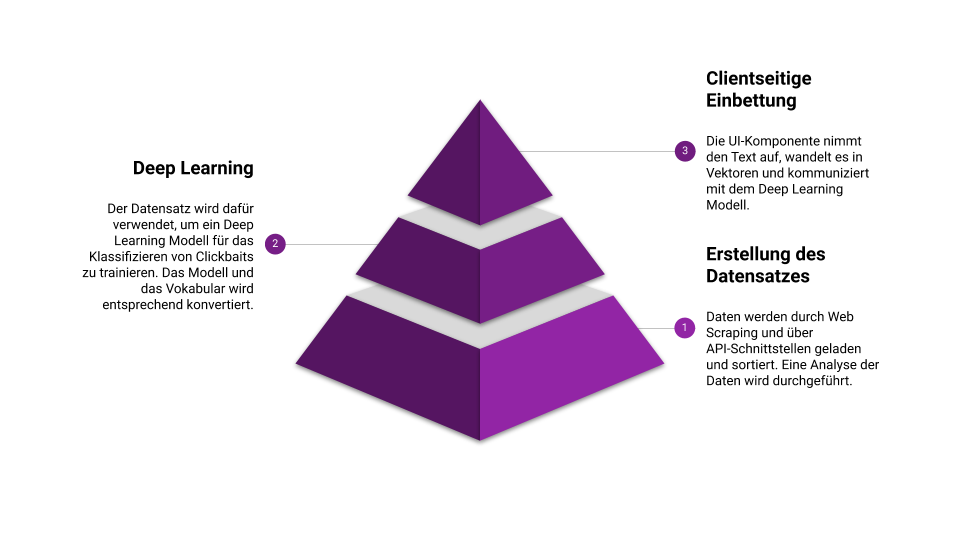
\includegraphics[width=15cm]{kapitel5/main_p.png}
    \caption[Darstellung der Konzeption]{Darstellung der Konzeption}
    \label{Kap5:Konzeption}
\end{figure}


Deep Learning Modelle benötigen eine große Menge an Beispielen um zu lernen. Es reicht außerdem nicht aus, nur eine große Menge an Daten zu beschaffen, sondern auch gute Daten auszuwählen. In der Studie von \cite*{Chakrabortya} haben die Autoren Daten aus dem Web geladen. Für die erste Kategorie, der Nicht-Clickbaits, wurde die Wikipedia-News-API verwendet. Um genug Beispiele für Clickbaits zu finden, sollten solche Medien herausgefunden werden. Um die Daten labeln zu können ist neben dem Titel eines Datenelementes auch die extraktion der Nachricht zu erfassen.

Die Wikipedia-News-API bietet einen Kostenlosen Endpunkt an, welches verschiedene Nachrichtenportale wie z.B. Politik, Wirtschaft, Kultur, Sport und Wissenschaft anbietet. Um Clickbaits zu finden verläuft die Datenaquise wesentlich schwieriger. Der Datensatz von \cite*{Chakrabortya} beinhalter jeweils 7500 Nachrichten je Kategorie. Es ist zu berücksichtigen, dass diese nicht mit Deep Learning Modellen arbeiten, sondern mit klassischen Machine Learning Algorithmen, die weniger Daten benötigen. Es müssen also mehr Daten her, also die Suche sollte neben den klassischen Clickbait-Seiten auch woanders erfolgen. Um die Datenextraktion zu automatisieren bietet sich die Software \enquote{Scrapy} an. Scrapy ist ein Open-Source Tool, welches das extrahieren von großen Mengen an Daten erleichtert. Es ist in Python geschrieben und kann durch seine Middleware Funktion auch die Daten direkt in eine SQL-Datenbank speichern.

Der mittlere Kern der Pyramide in Abbildung~\ref{Kap5:Konzeption} ist das Deep Learning Modell, welches als Inferenzmaschine betrachtet werden kann. Es wird durch Eingabe von gelabelten Daten trainiert und in ein entsprechendes Format gebracht. Es gibt mehrere Anbieter für das Deep Learning. Die meisten von Ihnen sind Open Source. Die bekanntesten Bibliotheken für das Deep Learning sind TensorFlow (welches von Google unterstützt wird) und PyTorch (welches von Facebook unterstützt wird). Seit März 2018 bietet TensorFlow die Möglichkeit, Modelle in der Programmiersprache JavaScript zu trainieren und zu benutzen. Ein klassischer Vorgang um Deep Learning Modelle dem Endbenutzer durch Webprogrammierung anzubieten war es immer, dass zunächst ein Modell trainiert wurde und dann auf einem Server geladen wurde. Der Server hatte dann einen Endpunkt, z.B. eine POST-Anfrage, welches eine Anfrage vom Clienten empfang. Diese Anfrage wurde dann im Server durch das Modell beantwortet und der Server sendete dem Clienten das Ergebnis. Durch TensorFlow.js ist es möglich erstens ein Modell komplett auf der Programmiersprache JavaScript zu entwickeln und zweitens es die Inferenzbildung durch einen Server in der Mitte nicht mehr nötig. Das Modell kann zusammen mit dem Framework in den Browser geladen werden und die bearbeitung erfolgt dort. In dieser Arbeit wurde das Modell nicht mit TensorFlow.js trainiert, da es auch möglich ist, Modelle in der konventionellen Weise mit der Keras API zu trainieren und dann in ein Webfreundliches Format umzuwandeln. Nach der Konversion können die Gewichte welches das Modell gerechnet hat und eine JSON-Datei, welches das Modell beschreibt hochgeladen und benutzt werden. Der Client muss nur noch diese Dateien in den Browser laden und kann dann selbst die Anfrage beantworten. Das trainieren auf konventionellen Wegen bietet außerdem den Vorteil, dass die Umgebung auf JavaScript nicht mit der Umgebung in Python konkurrieren kann. Die meisten Tools und Frameworks werden für Python geschrieben. Ein weiterer Grund ist, dass die bearbeitung auf dem heimischen Computer sehr langsam ist. Mit Google Colab können Deep Learning Modelle mit viel Rechnerkapazität trainiert werden.

Die Spitze der Pyramide macht die Benutzeroberfläsche aus. Diese wird komplett in JavaScript geschrieben. JavaScript ist die meistbenutze Programmiersprache und wird heute neben Webentwicklung auch auf dem Server verwendet. Mit TensorFlow.js ist es nun auch möglich, mit Tensors umzugehen. Die Schwierigkeit hier ist es, den Text, den der Benutzer eingibt, in Token und dann diese Token in Vektoren umzuwandeln, wenn das Modell keinen sogenannten \enquote{Input-Layer} hat welches einfache String einnehmen kann und diese umwandeln kann, dieses macht das Modell aber viel größer, da es eine größere Anzahl an Parametern hat und nicht Ziel dieser Arbeit. Eine andere Möglichkeit ist es, das gesamte Vokabular in einer JSON-Datei zu speichern und es der Benutzeroberfläsche zugänglich zu machen. Jedes auftauchende Wort im Vokabular bekommt einen Index, welches dann als \enquote{Übersetzer} dient und zur Umwandlung der Strings in Vektoren verwendet werden.




\section{Erstellung des Datensatzes}
\subsection{Erste Rohdatenbeschaffung durch Web Scraping}

Um einen Forschungsbeitrag zu leisten, hat diese Arbeit das Ziel ein Clickbait Corpus auf deutscher Sprache zu erstellen. Für die Erstellung eines solchen Korpus sind zunächst bestimmte Seiten einzugrenzen, die Clickbait Nachrichten anbieten. Die bekannteste Seite ist \enquote{buzzfeed} und \enquote{tasty}. Außerdem wurden auch Webseiten wie \enquote{web.de} oder \enquote{tv-movie}\footnote{Beinhaltet außerdem Schlagzeilen aus den Bereichen \enquote{tasty} und \enquote{quiz}} nach Clickbaits gescannt. Das Screening wurde am November 2020 durchgeführt. Um jedoch zu gewährleisten, dass die Nachrichten zeitlich weit außereinder liegen und somit eine größere Diversität haben, wurden Webseiten ausgewählt die Ihre Nachrichten in gewisser Weise Archivieren. Die gesammelten Daten reichen teilweise über ein Jahr zurück. Wie im Listing~\ref{Scrapy} unter in Zeile 12 zu sehen ist, besitzt die Seite im Beispiel eine Pagination-Funktion. Diese kann dafür verwendet werden, um auch ältere Nachrichten zu erfassen.

\begin{table}[h]
    \caption{Vergleich der Rohdaten nach dem Scrapingvorgang}
    \label{Datensatz_Herkunft}
    \renewcommand{\arraystretch}{1.2}
    \centering
    \sffamily
    \begin{footnotesize}
        \begin{tabular}{l l l}
            \toprule
            \textbf{Quelle}   & \textbf{Methodik} & Elemente \\
            \midrule
            de.wikinews.org   & API-Zugang        & 10.612   \\
            web.de            & Web Scraping      & 14.163   \\
            tvmovie.de        & Web Scraping      & 9.428    \\
            buzzfeed.de       & Web Scraping      & 798      \\
            promipool.de      & Web Scraping      & 26.779   \\
            heftig.de         & Web Scraping      & 605      \\
            frauenseite.net   & Web Scraping      & 148      \\
            bravo.de          & Web Scraping      & 7.476    \\
            \midrule
            Summe Clickbaits  &                   & 59.407   \\
            Summe Nachrichten &                   & 10.612   \\
            Summe insgesamt   &                   & 70.019   \\
            \bottomrule
        \end{tabular}
    \end{footnotesize}
    \rmfamily
\end{table}



Das Verfahren wurde automatisch mittels eines programmierten Scrapers je Seite durchgeführt. Ein Scraper ist ein Programm, welches Informationen aus einer Webseite automatisch extrahieren kann. Dieses gelingt, indem es nach HTML- oder CSS-Attributen oder sogar AJAX-Requests durchsucht oder diese imitiert. Im Listing~\ref{Scrapy} wird ein Web-Scraper vorgestellt. Scrapy führt in einer Schleife HTTP-Requests durch welche jeweils eine Antwort bekommen. Es können auch AJAX-Anfragen gesendet werden (z.B. ein POST-Request). Wenn die Anfrage Erfolgreich ist, kann die daraus resultierende Antwort auf bestimmte Eigenschaften und Attribute durchsucht werden (im Beispiel werden CSS-Attribute durchsucht). Diese Attribute beinhalten meisten die gewünschte Information, welches dann wie in der \texttt{parse\_url} und \texttt{parse\_page} Methode gezogen und in eine Datenbank gespeichert wird.



\begin{lstlisting}[language=Python,caption=Beispiel eines Scrapers]
import scrapy
from scrapy.http.request import Request
from datetime import datetime
from klickscraper.items import WebdeItem


class WebdeSpider(scrapy.Spider):
    name = "webde"
    scraped_at = datetime.now()

    def start_requests(self):
        for i in range(287):
            url = f"https://web.de/magazine/unterhaltung/stars/p{i}"
            yield Request(
                dont_filter=True,
                callback=self.parse_url,
                url=url)

    def parse_url(self, response):
        follow_ulrs = response.css(
            ".teaser-article__full").css("a::attr(href)").getall()
        for f in follow_ulrs:
            yield Request(
                url=f,
                dont_filter=True,
                callback=self.parse_page)

    def parse_page(self, response):
        if len(response.css("p::text").getall()) > 10:
            text = " ".join(response.css("p::text").getall())
        else:
            text = None
        yield WebdeItem(title=response.css('title::text').get(),
                        text=text,
                        scraped_at=self.scraped_at)
\end{lstlisting}\label{Scrapy}


\subsection{Explorative Datenanalyse der Rohdaten}
Um aus den Rohdaten Schlüsse über die sprachlichen Eigenschaften zu ziehen wird im folgenden Abschnitt eine explorative Datenanalyse durchgeführt. Um dies möglichst zu vereinfachen, wird der Rohdatensatz welches in einer SQL-Datenbank gespeichert wurde in ein Pandas\footnote{Pandas ist ein schnelles, flexibles und benutzerfreundliches Open-Source-Tool zur Analyse und Bearbeitung von Daten in Python.} Dataframe umgewandelt.
Aus der Abbildung~ist zu sehen, dass die Titel aus Wikinews länger sind. Neben der Länge der Schlagzeilen ist auch die Analyse der Wortauswahl wichtig. Aus der Literaturstudie können bestimmte Merkmale von Clickbaits festgestellt werden. Clickbaits enthalten meistens eine Frage oder Zahlen. Außerdem ist bei Clickbaits auch eine gewisse Wortauswahl festzustellen. Die Zuordnung der Wörter je Clickbait-Schlagzeile zu den Wortarten (Part-of-speech-Tagging oder POS-Tagging) wurde mittels der Python NLP-Bibliothek Spacy durchgeführt. Bei der Auswahl der Tags nachdem gesucht werden sollte, wurden die Erkenntnisse aus Kapitel 4 Berücksichtigt. Die Ergebnisse diese Analyse sind aus der Tabelle~\ref{pos} zu entnehmen.

\begin{table}[h]
    \caption{Vergleich der Ergebnisse des Part-of-speech-Taggings}
    \label{pos}
    \renewcommand{\arraystretch}{1.2}
    \centering
    \sffamily
    \begin{footnotesize}
        \begin{tabular}{l l l}
            \toprule
            \textbf{TAG}                  & \textbf{Auffälliges Wort (Häufigkeit)} \\
            \midrule
            ADJA  (attributives Adjektiv) & neu (1759), neue (1474)                \\
            ADJD   (adverbiales Adjektiv) & krass (171), wirklich  (349)           \\
            ADV   (Adverb)                & so (5142), endlich (357)               \\
            PDAT (Demonstrativpronomen)   & dies (3566)                            \\
            PROAV   (Pronominaladverb)    & darum (588), deshalb (251)             \\
            PWAT (Interrogativpronomen)   & welch (154)                            \\
            PWAV  (Relativpronomen)       & wie (488) warum (184)                  \\
            \bottomrule
        \end{tabular}
    \end{footnotesize}
    \rmfamily
\end{table}

% Eine eigene Analyse durch das Part-of-Speech_tagging mittels Scrapy ergibt einige Auffälligkeiten bezüglich der Clickbaits. Wörter wie \enquote{diese} (attribuierendes Demonstratives Pronomen), \enquote{warum} (adverbiales Interrogativ- oder Relativpronomen) oder \enquote{welche} (attribuierendes Interrogativpronomen) sind einige Auffällige Tags aus den Schlagzeilen der Clickbaits.



% \begin{lstlisting}[language=Python,caption=Funktion zur Umwandung der Datenbank in en Pandas Dataframe]
% def connect_to_db(tablename, db_path):
%     return pd.read_sql_query(
%         f"SELECT * FROM {tablename}", sqlite3.connect(db_path))
% \end{lstlisting}\label{Pandasdb}


\begin{figure}[H]
    \centering
    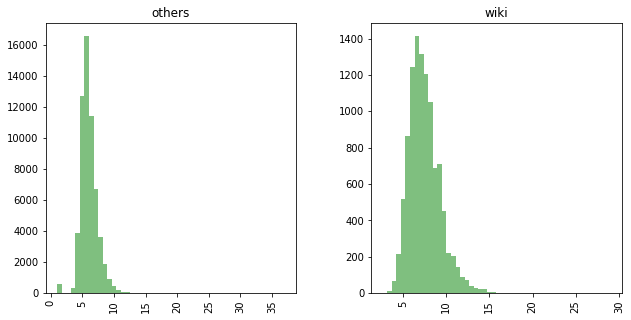
\includegraphics[width=14cm]{kapitel5/hist2.png}
    \caption[Vergleich der Wortlängen der Rohdaten]{Vergleich der Wortlängen, das Histogramm rechts (Wikinews) ist breiter als das Histogramm links (Clickbaits)}
    \label{Kap5:Hist2}
\end{figure}

% \begin{figure}[H]
%     \centering
%     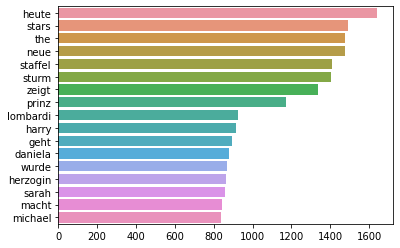
\includegraphics[width=10cm]{kapitel5/freq_word1.png}
%     \caption[Häufigsten Wörter aus den Rohdaten der Clickbaits Titel]{Die Darstellung zeigt das Aufkommen der Häufigsten Wörter aus den Titeln der Clickbaits}
%     \label{Kap5:freq1}
% \end{figure}

% \begin{figure}[H]
%     \centering
%     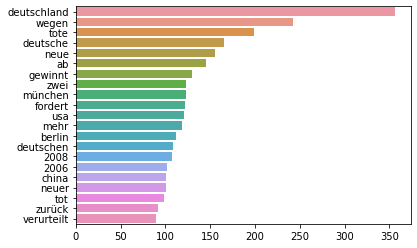
\includegraphics[width=10cm]{kapitel5/freq_word2.png}
%     \caption[Häufigsten Wörter aus den Rohdaten der Wikinews Titel]{Die Darstellung zeigt das Aufkommen der Häufigsten Wörter aus den Titeln der Wikinews Nachrichten}
%     \label{Kap5:freq2}
% \end{figure}


\subsection{Labeln der Daten}
Aus der Tabelle~\ref{Datensatz_Herkunft} ist zu entnehmen, dass ca. 60.000 potenzielle Clickbaits vorhanden sind. Um dieses nicht per Hand labeln zu müssen besteht der Ansatz darin, bestimmte Muster zu erkennen und diese Muster auszunutzen, um die Anzahl der Kandidaten auf ein entsprechendes niedriges Niveau zu bringen. Die Literaturstudie und die explorative Datenanalyse bringen gemeinsam folgende Schlüsse:

\begin{enumerate}
    \item Clickbaits sind meisten Fragen wie \enquote{Welcher Schuh passt dir am meisten?}
    \item Clickbaits enthalten meistens Zahlen in Form eines Listings \enquote{Das sind die 10 schnellsten Autos}
    \item Clickbaits haben eine niedrigere Wortlänge als normale Nachrichten
    \item Clickbaits beinhalten einige für sie markanten Wörter wie \enquote{diese} oder \enquote{so}
\end{enumerate}

Diese Erkenntnisse können programmatisch umgewandelt werden und somit der Rohdatensatz um ein vielfaches reduziert werden.


\begin{lstlisting}[language=Python,caption=Funktion welches ein Dataframe je nach Argumenten labelt]
def contains_word(word, row):
    for r in row:
        if r in word:
            return 1


def label_data_with_arg(df, col_name, arg_):
    return df[col_name].apply(
        lambda x: contains_word(arg_, re.findall(r"[\w']+|[.,!?;]", x.lower())))
\end{lstlisting}\label{Label1}

\begin{lstlisting}[language=Python,caption=Funktionen für durchschnittliche Wortlänge und Interpunktion]
import re
import string

def remove_punc(text):
    text = re.sub('\[.*?\]', '', text)
    text = re.sub('https?://\S+|www\.\S+', '', text)
    text = re.sub('<.*?>+', '', text)
    text = re.sub('[%s]' % re.escape(string.punctuation), '', text)
    text = re.sub('\n', '', text)
    text = re.sub('\w*\d\w*', '', text)
    return text

def get_avg_length(string):
    words = remove_punc(string).split()
    try:
        count = int(sum(len(word) for word in words) / len(words))
    except ZeroDivisionError:
        count = 1
    return count
\end{lstlisting}\label{Label2}

\begin{lstlisting}[language=Python,caption=Tagger Funktion]
import spacy
nlp = spacy.load('de')

def contains_pos(sentence):
    list_ = ["PDAT", "ADJD", "ADJA", "PIS", "PWAV", 
            "PTKA", "VAFIN", "PROAV", "ADV"]
    doc = nlp(sentence)
    for token in doc:
        if str(token.tag_) in list_:
            return "1"

def label_data_with_pos(df, col_name):
    return df[col_name].apply(
        lambda x: contains_pos(x.lower()))
\end{lstlisting}\label{Label3}


\subsection{Analyse der Daten}
Die Summe der Wikinews Nachrichten beträgt ca. 10.000. Mit der Zugabe weiterer 10.000 Clickbaits, die durch das labeln entstehen, ergibt sich ein Datensatz mit 20.000 Beispielen. Die Tabelle~\ref{data} verschafft einen Übrerblick über alle Daten. Interessant ist bei den Clickbaits, dass ca. 33\% aller Clickbaits ein Fragezeichen oder eine Zahl beinhalten und ca. die hälfte aller Daten im Datensatz ein bestimmtes Tag wie \enquote{diese} oder \enquote{so} enthalten. Bei den Wikinews Nachrichten liegen diese Anteile deutlich unten. Alle drei genannten Eigenschaften liegen unter 1\%. Die durchscnittliche Wortlänge beträgt bei den Clickbaits bei 5, während bei den Wikipedia Nachrichten dieses bei 7 liegt.

\begin{table}[h]
    \caption{Beschreibung des gelabelten Datensatzes}
    \label{data}
    \renewcommand{\arraystretch}{1.2}
    \centering
    \sffamily
    \begin{footnotesize}
        \begin{tabular}{l l l l l l}
            \toprule
                           & \textbf{has\_question} & \textbf{has\_keyword} & \textbf{has\_number} & \textbf{avg\_word\_length} & \textbf{label} \\
            \textbf{count} & 20000                  & 20000                 & 20000                & 20000                      & 20000          \\
            \textbf{mean}  & 0.1782                 & 0.3190                & 0.0854               & 6.1307                     & 0.5000         \\
            \textbf{std}   & 0.3826                 & 0.4661                & 0.2795               & 1.7874                     & 0.5000         \\
            \textbf{min}   & 0                      & 0                     & 0                    & 1.0000                     & 0              \\
            \textbf{max}   & 1                      & 1                     & 1                    & 27.0000                    & 1              \\

            \bottomrule
        \end{tabular}
    \end{footnotesize}
    \rmfamily
\end{table}

Bei der Betrachtung der Wörter mit der Word-Cloud Analyse können bestimmte Themen, die die Titel zürückgeben betrachtet werden.  Auffällig sind neben Promis auch die Wörter \enquote{darum}, \enquote{quiz} \enquote{sieht} und \enquote{macht}. Bei den Wikipedia Nachrichten geht es mehr um Deutschland und der Welt.


\begin{figure}[H]
    \centering
    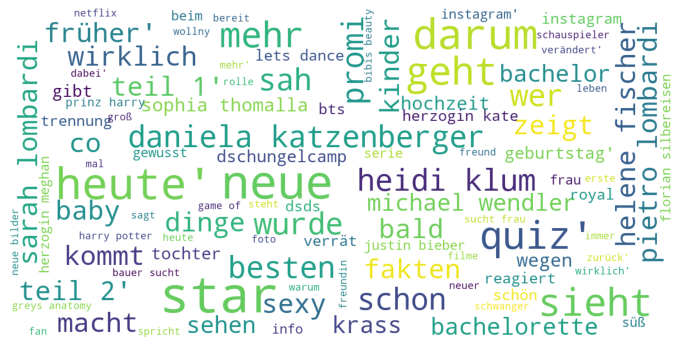
\includegraphics[width=12cm]{kapitel5/wo_click.png}
    \caption[Word Cloud Analyse für die Clickbaits Schlagzeilen]{Die Darstellung zeigt das Aufkommen der Häufigsten Wörter aus den Titeln der Wikinews Nachrichten}
    \label{Kap5:clwc}
\end{figure}

\begin{figure}[H]
    \centering
    \includegraphics[width=12cm]{kapitel5/news.png}
    \caption[Word Cloud Analyse für die Wikinews Schlagzeilen]{Die Darstellung zeigt das Aufkommen der Häufigsten Wörter aus den Titeln der Wikinews Nachrichten}
    \label{Kap5:clwc}
\end{figure}

 % Externe Datei einbinden
% ------------------------------------------------------------------

\label{lastpage}

% Neue Seite
\cleardoublepage

% Backmatter mit normalem Zeilenabstand setzen
\singlespacing

% Römische Ziffern für die "Back-Matter", fortlaufend mit "Front-Matter"
\pagenumbering{roman}
\setcounter{page}{\value{frontmatterpage}}

% Abkürzungsverzeichnis
\addchap{\hsmaabbreviations}
% % Die längste Abkürzung kann in die eckigen Klammern
% % bei \begin{acronym} geschrieben, um einen hässlichen
% % Umbruch zu verhindern
% %
% % ACHTUNG: Sie müssen die Abkürzungen von Hand alphabetisch
% %          sortieren. Das passiert nicht automatisch.
% \begin{acronym}[IEEE]
% \acro{ABK}{Abkürzung}
% \acro{ACM}{Association of Computing Machinery}
% \acro{PDF}{Portable Document Format}
% \acro{IEEE}{Institute of Electrical and Electronics Engineers}
% \acro{ISO}{International Organization for Standardization}
% \end{acronym}


% Tabellenverzeichnis erzeugen
\cleardoublepage
\phantomsection
\addcontentsline{toc}{chapter}{\hsmalistoftables}
\listoftables

% Abbildungsverzeichnis erzeugen
\cleardoublepage
\phantomsection
\addcontentsline{toc}{chapter}{\hsmalistoffigures}
\listoffigures

% Listingverzeichnis erzeugen. Wenn Sie keine Listings haben,
% entfernen Sie einfach diesen Teil.
\cleardoublepage
\phantomsection
\addcontentsline{toc}{chapter}{\hsmalistings}
\lstlistoflistings

% Literaturverzeichnis erzeugen
\begingroup
\cleardoublepage
\begin{flushleft}
    \let\clearpage\relax % Fix für leere Seiten (issue #25)
    \printbibliography
\end{flushleft}
\endgroup

% Index ausgeben. Wenn Sie keinen Index haben, entfernen Sie einfach
% diesen Teil. Die meisten Abschlussarbeiten haben *keinen* Index.
\cleardoublepage
\phantomsection
\addcontentsline{toc}{chapter}{\hsmaindex}
\printindex

% Anhang. Wenn Sie keinen Anhang haben, entfernen Sie einfach
% diesen Teil.
\appendix
% \chapter{Erster Anhang}

% Hier ein Beispiel für einen Anhang. Der Anhang kann genauso in Kapitel und Unterkapitel unterteilt werden, wie die anderen Teile der Arbeit auch.

% \chapter{Zweiter Anhang}

% Hier noch ein Beispiel für einen Anhang.


\end{document}
